% ---------------- APENDICE A ----------------
\clearpage
\onecolumn
\section*{Apéndice A. Evidencia gráfica del proceso experimental}
\pendiente{Mencionar en el texto}{Citar el Apéndice A en III.3 y III.4 (p.~ej. «véanse las Figuras A1 a A7») y precisar en qué consisten los «puntos de tensión» definidos en Fusion 360 (¿carga, apoyo o ambos?).}
\begingroup\setcounter{figure}{0}\renewcommand{\thefigure}{A\arabic{figure}}
\begin{figure}[!htbp]\centering
\begin{subfigure}[t]{0.48\textwidth}\centering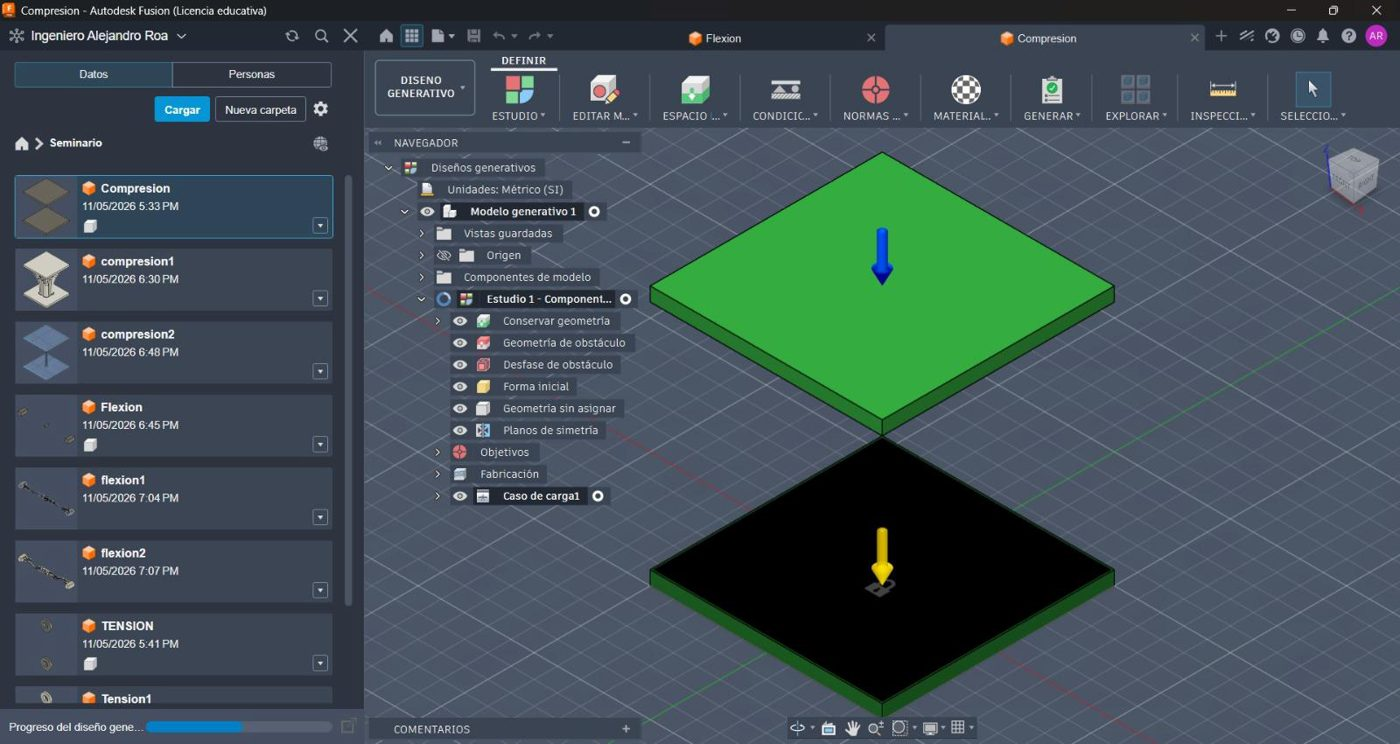
\includegraphics[width=\linewidth,height=0.20\textheight,keepaspectratio]{anexo/p13_0.jpg}\end{subfigure}\hfill
\begin{subfigure}[t]{0.48\textwidth}\centering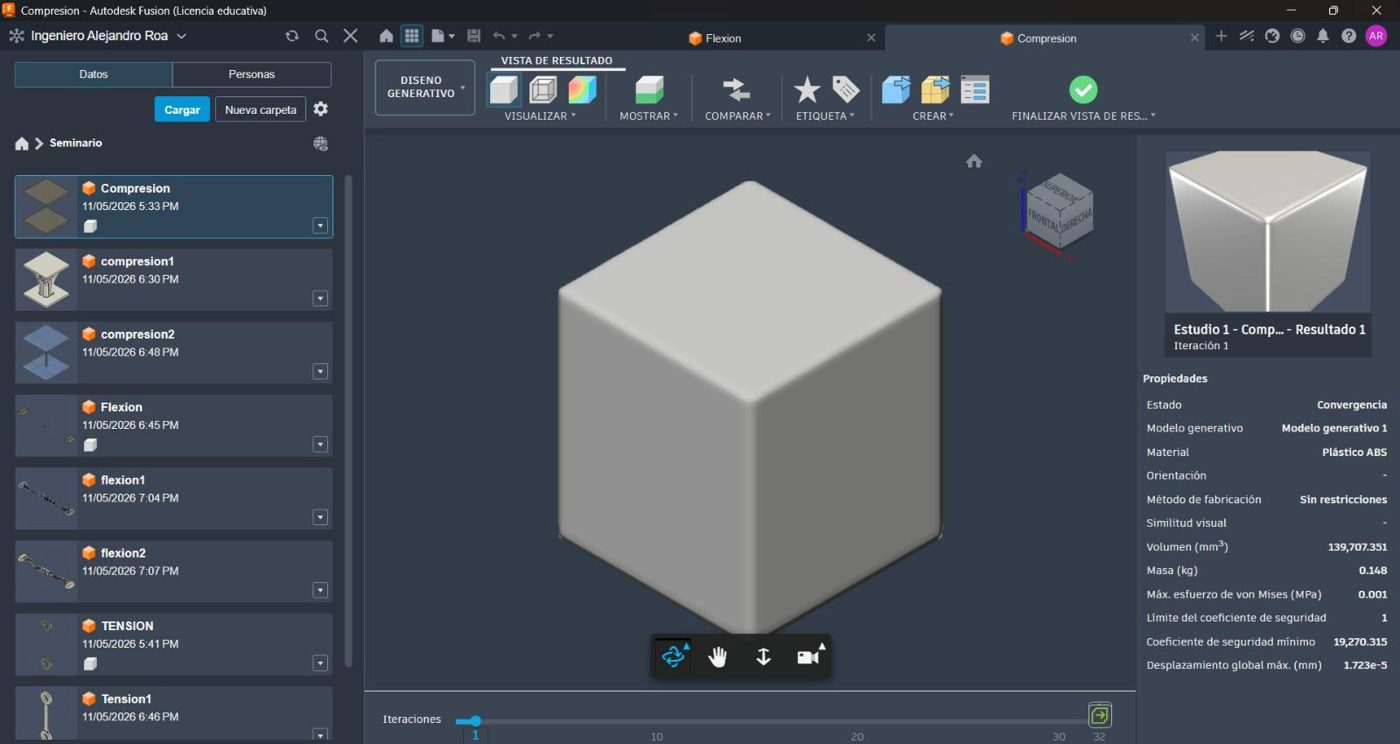
\includegraphics[width=\linewidth,height=0.20\textheight,keepaspectratio]{anexo/p13_1.jpg}\end{subfigure}\par\smallskip
\begin{subfigure}[t]{0.48\textwidth}\centering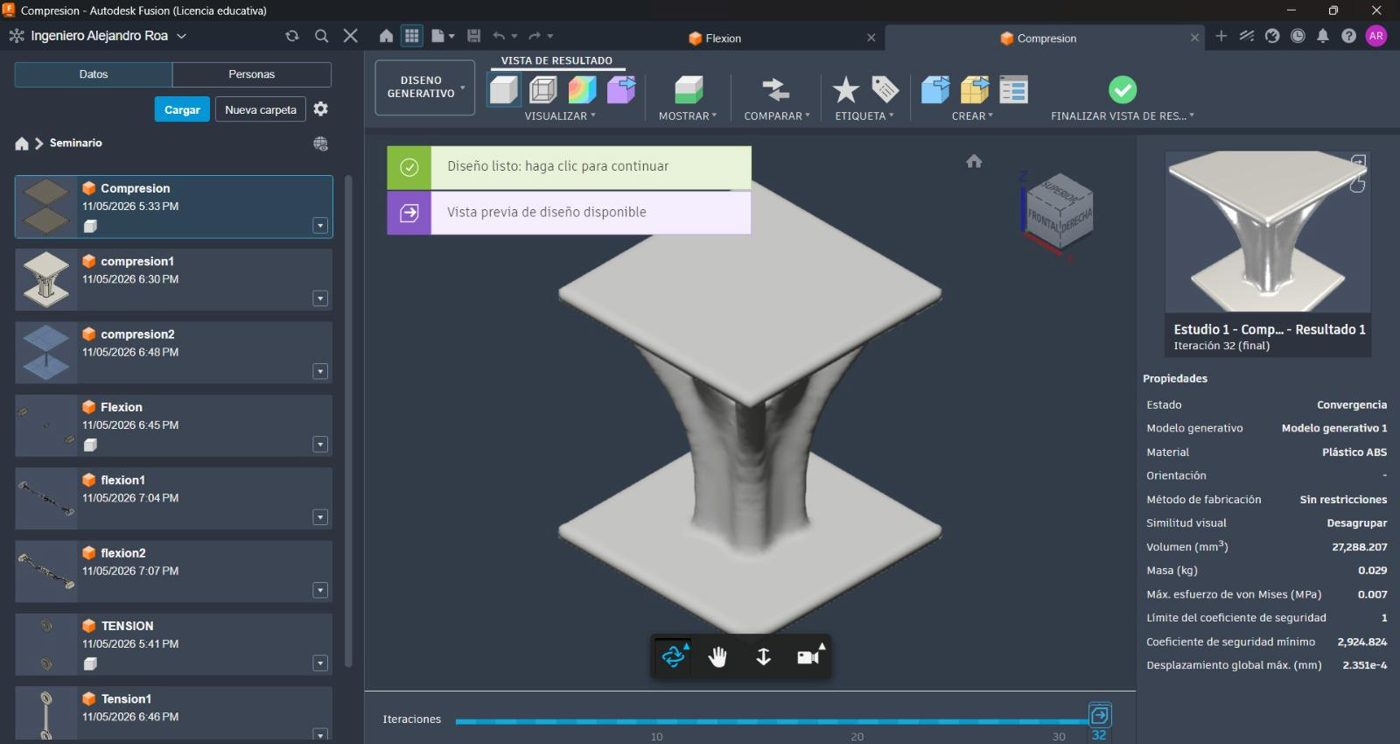
\includegraphics[width=\linewidth,height=0.20\textheight,keepaspectratio]{anexo/p14_0.jpg}\end{subfigure}\hfill
\begin{subfigure}[t]{0.48\textwidth}\centering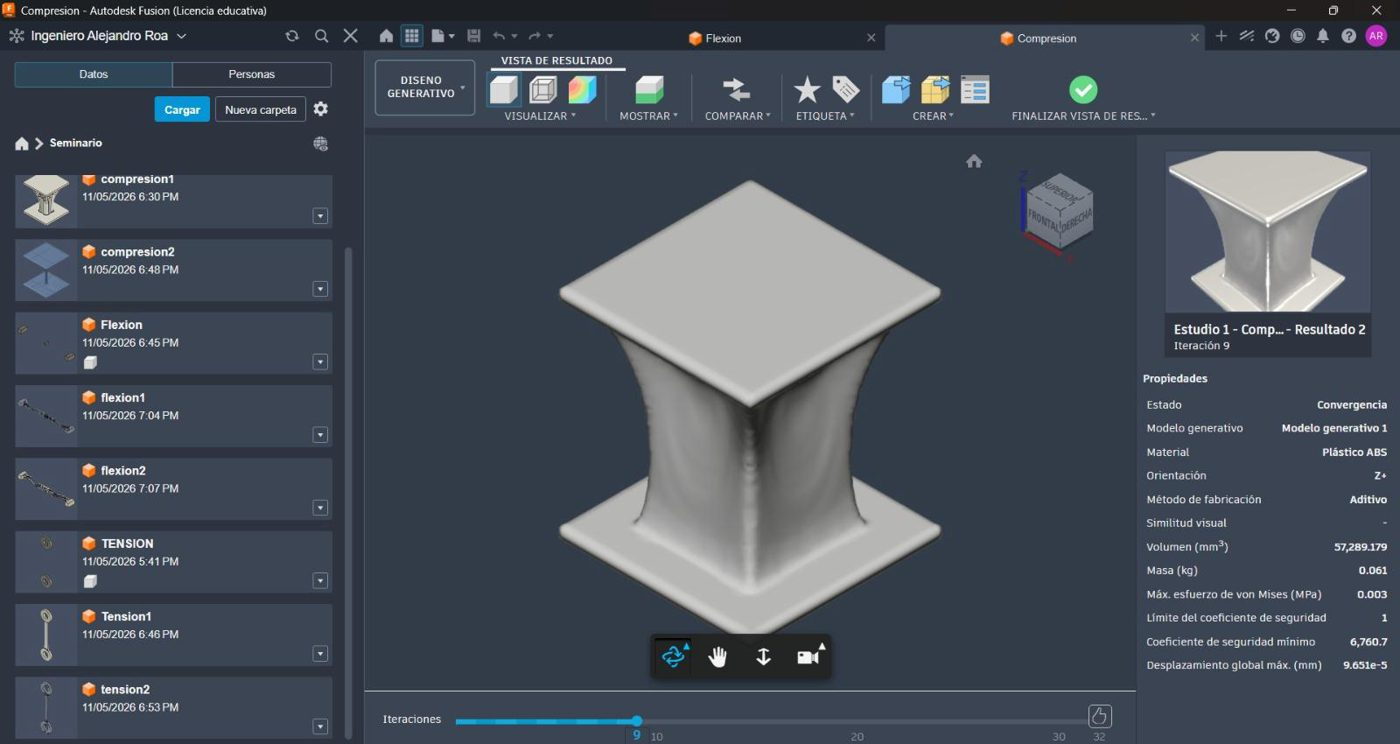
\includegraphics[width=\linewidth,height=0.20\textheight,keepaspectratio]{anexo/p14_1.jpg}\end{subfigure}\par\smallskip
\begin{subfigure}[t]{0.48\textwidth}\centering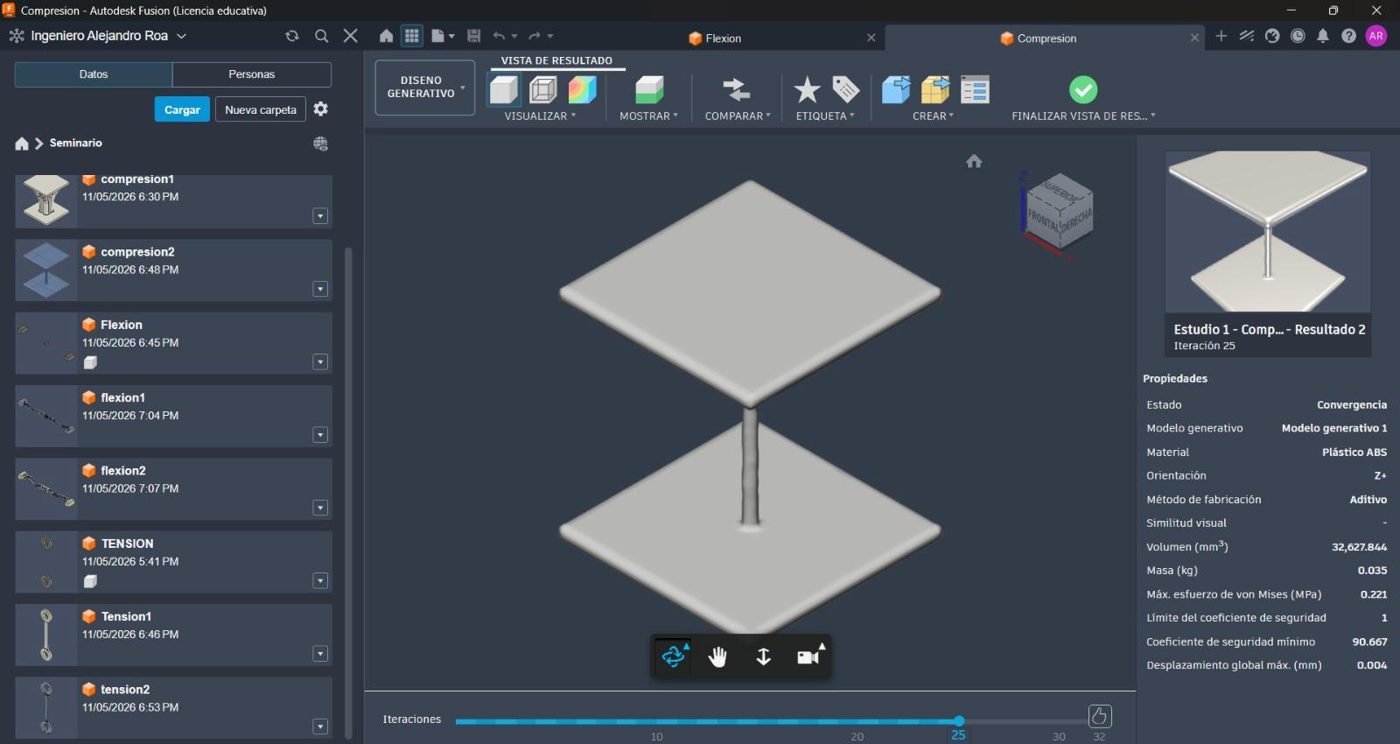
\includegraphics[width=\linewidth,height=0.20\textheight,keepaspectratio]{anexo/p15_0.jpg}\end{subfigure}\hfill
\begin{subfigure}[t]{0.48\textwidth}\centering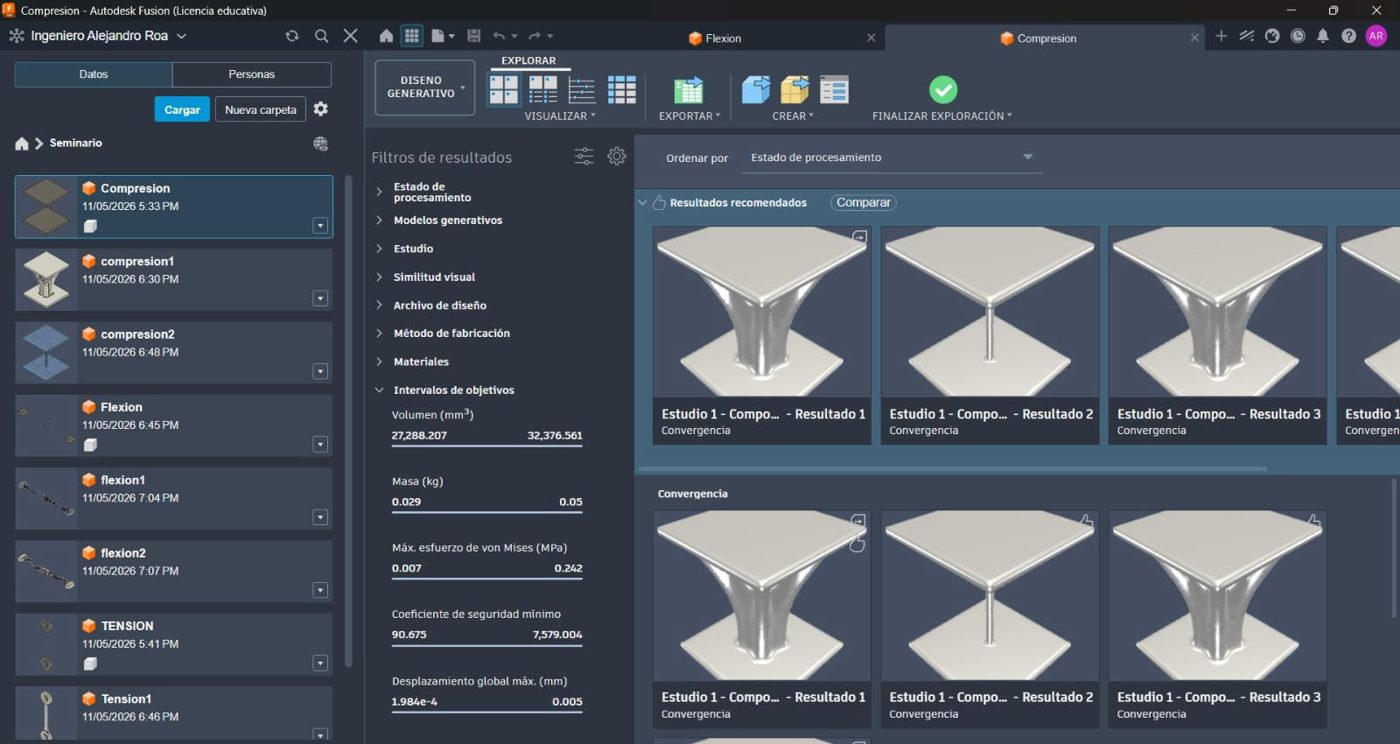
\includegraphics[width=\linewidth,height=0.20\textheight,keepaspectratio]{anexo/p15_1.jpg}\end{subfigure}\par\smallskip
\caption{Diseño generativo de la pieza de compresión en Fusion 360: definición de geometrías y cargas, espacio de diseño inicial, alternativas generadas y comparación de resultados.}
\par\footnotesize\textit{Nota.} Elaboración propia. Documento original, páginas 13 a 15.
\end{figure}
\begin{figure}[!htbp]\centering
\begin{subfigure}[t]{0.48\textwidth}\centering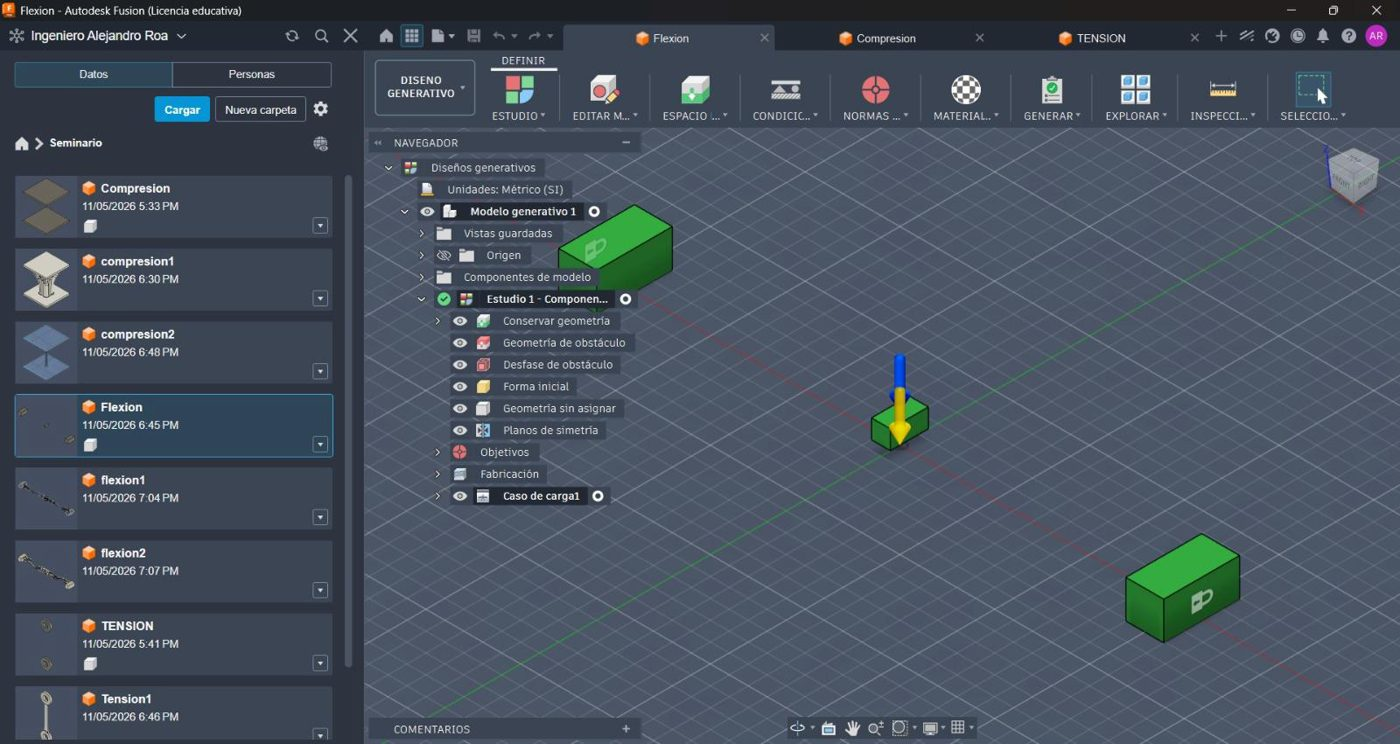
\includegraphics[width=\linewidth,height=0.20\textheight,keepaspectratio]{anexo/p18_1.jpg}\end{subfigure}\hfill
\begin{subfigure}[t]{0.48\textwidth}\centering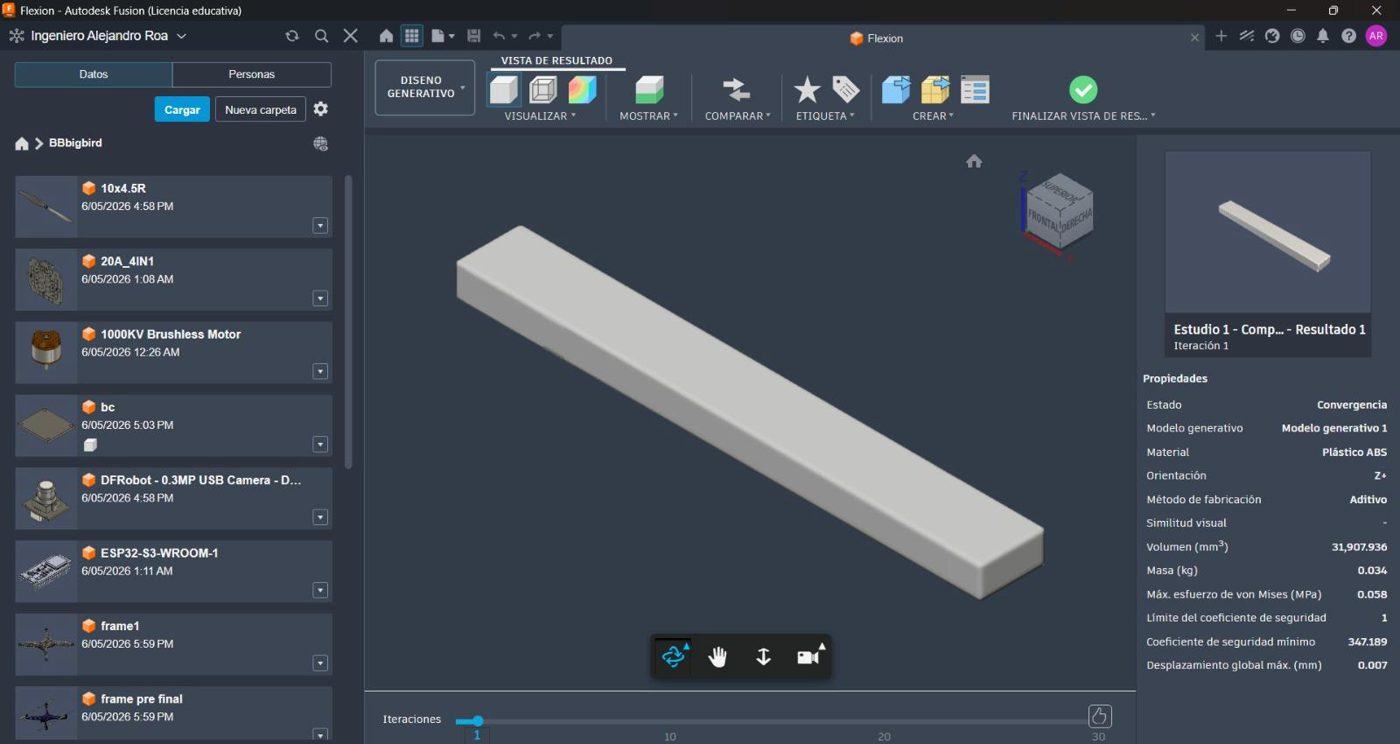
\includegraphics[width=\linewidth,height=0.20\textheight,keepaspectratio]{anexo/p16_0.jpg}\end{subfigure}\par\smallskip
\begin{subfigure}[t]{0.48\textwidth}\centering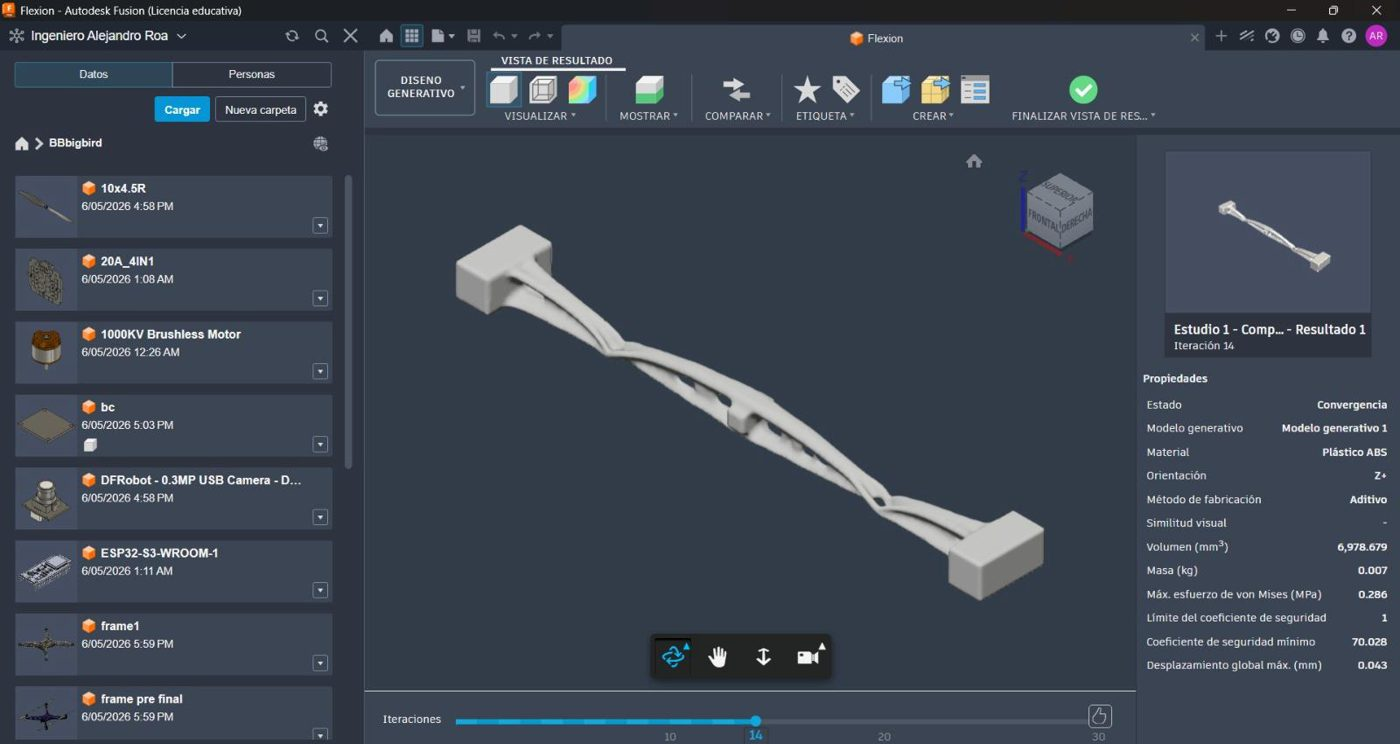
\includegraphics[width=\linewidth,height=0.20\textheight,keepaspectratio]{anexo/p16_1.jpg}\end{subfigure}\hfill
\begin{subfigure}[t]{0.48\textwidth}\centering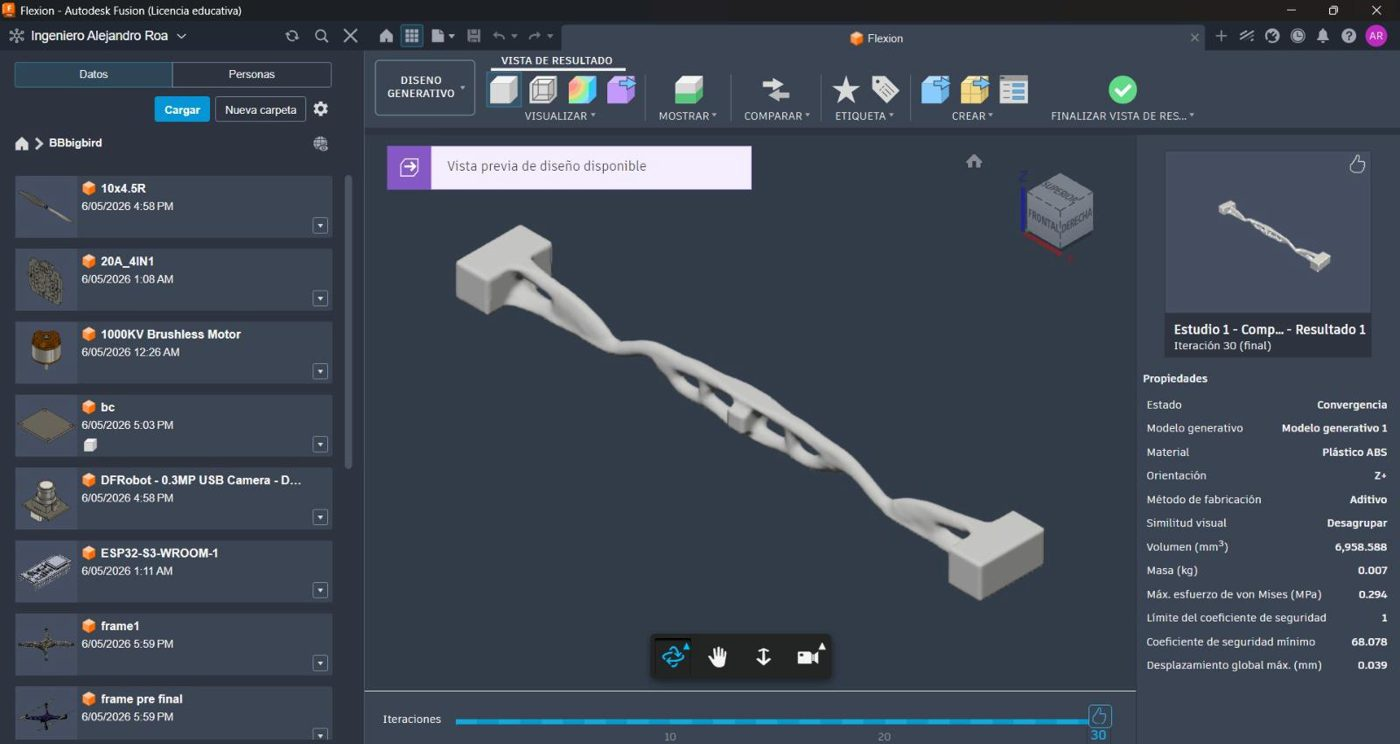
\includegraphics[width=\linewidth,height=0.20\textheight,keepaspectratio]{anexo/p17_0.jpg}\end{subfigure}\par\smallskip
\begin{subfigure}[t]{0.48\textwidth}\centering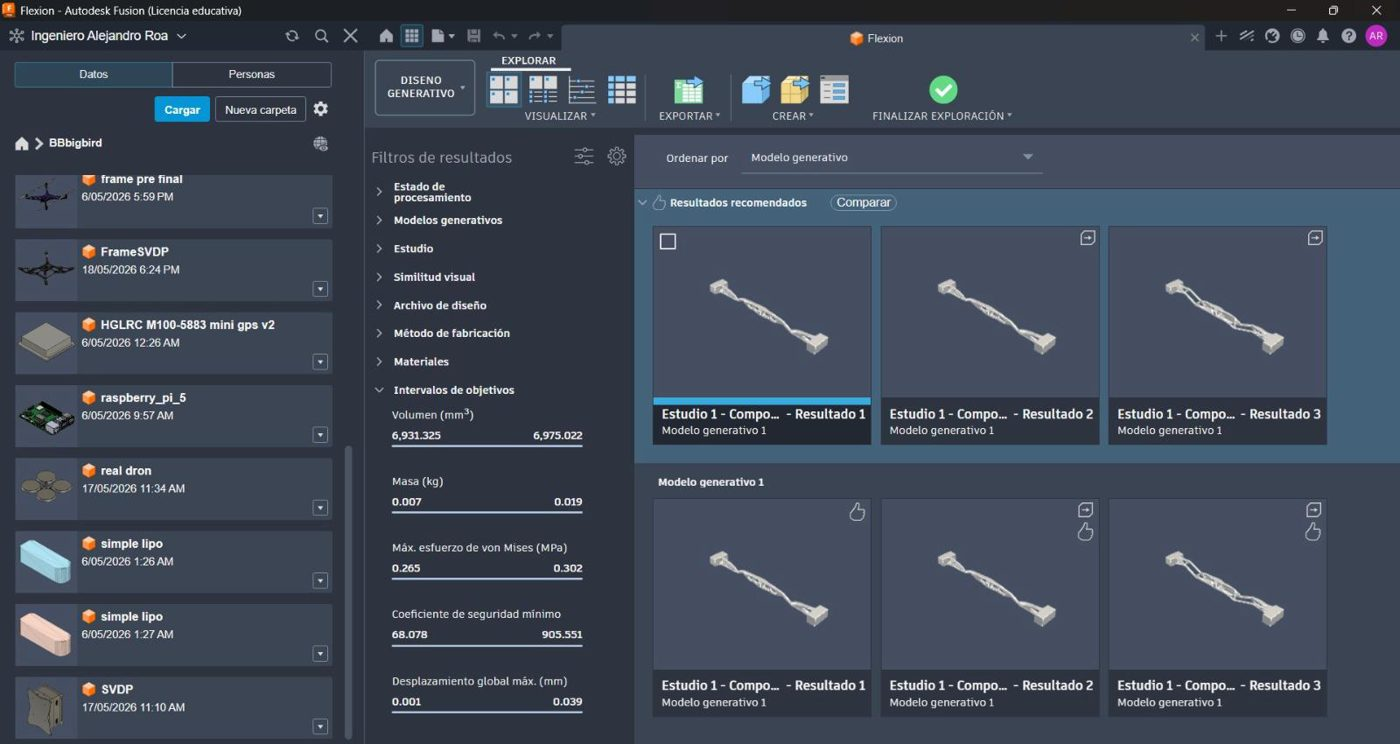
\includegraphics[width=\linewidth,height=0.20\textheight,keepaspectratio]{anexo/p17_1.jpg}\end{subfigure}\hfill
\caption{Diseño generativo de la pieza de flexión en Fusion 360: definición de geometrías y cargas, forma inicial y alternativas generadas.}
\par\footnotesize\textit{Nota.} Elaboración propia. Documento original, páginas 16 a 18.
\end{figure}
\begin{figure}[!htbp]\centering
\begin{subfigure}[t]{0.48\textwidth}\centering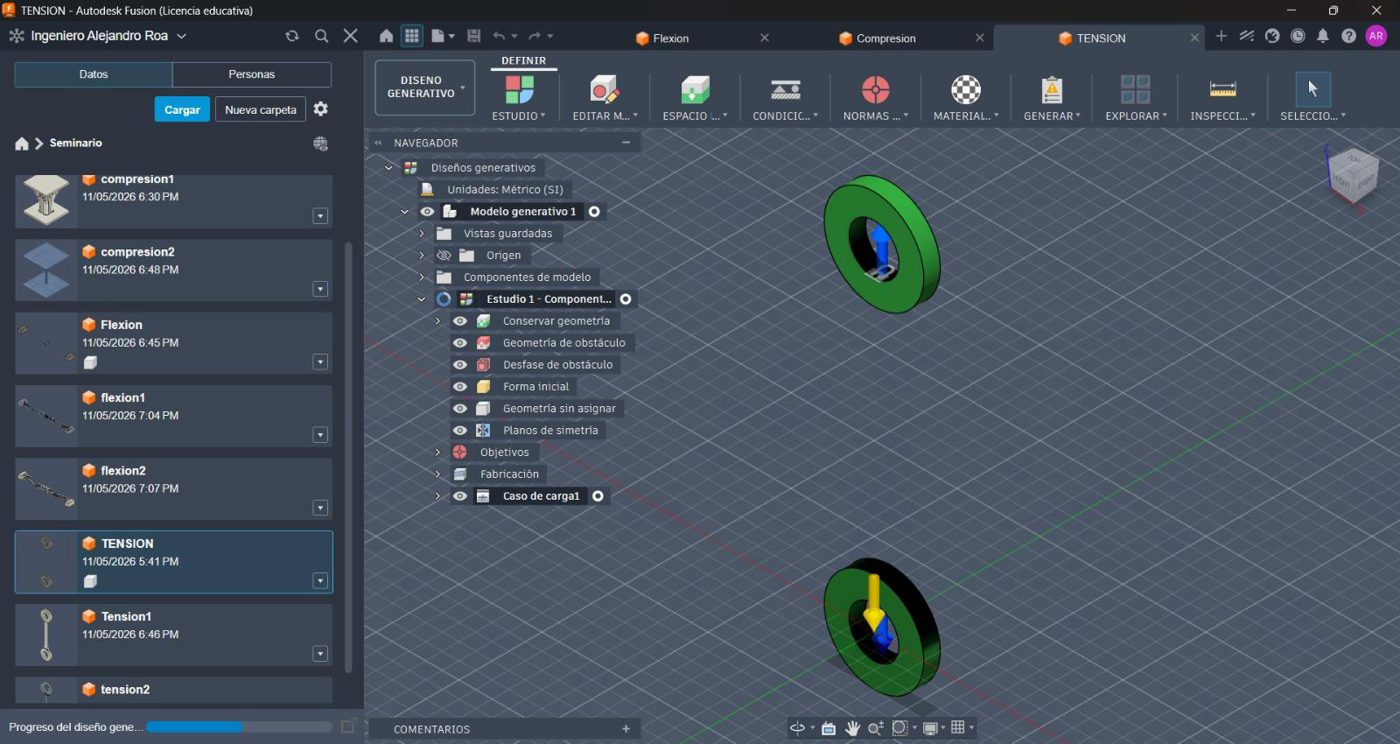
\includegraphics[width=\linewidth,height=0.20\textheight,keepaspectratio]{anexo/p18_0.jpg}\end{subfigure}\hfill
\begin{subfigure}[t]{0.48\textwidth}\centering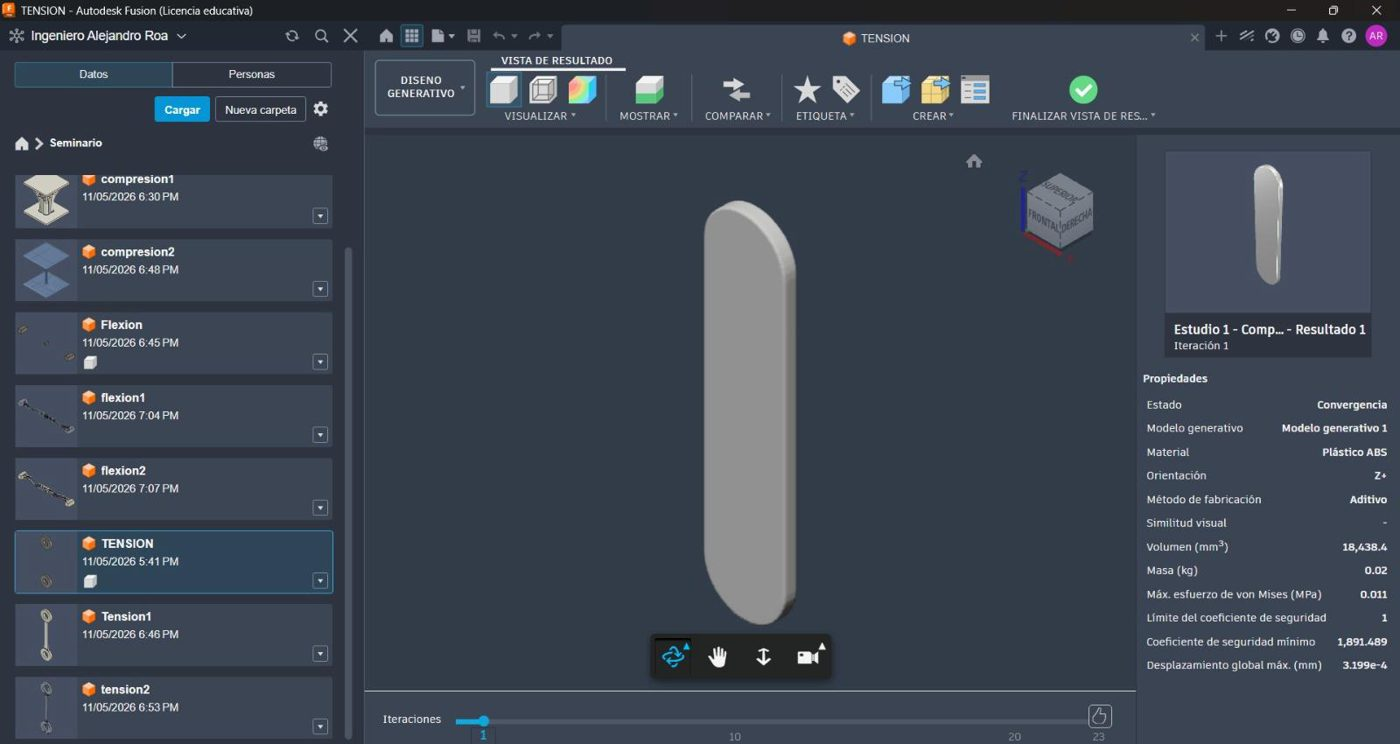
\includegraphics[width=\linewidth,height=0.20\textheight,keepaspectratio]{anexo/p19_0.jpg}\end{subfigure}\par\smallskip
\begin{subfigure}[t]{0.48\textwidth}\centering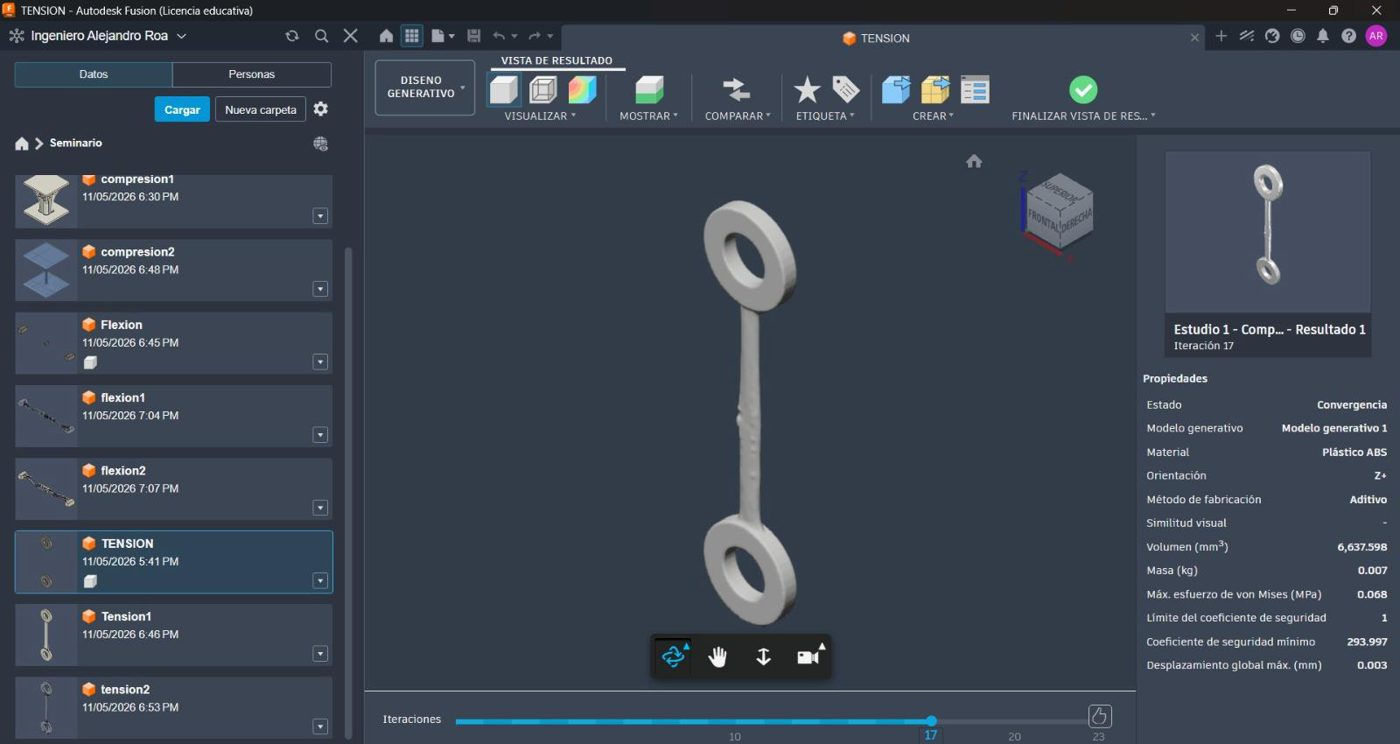
\includegraphics[width=\linewidth,height=0.20\textheight,keepaspectratio]{anexo/p19_1.jpg}\end{subfigure}\hfill
\begin{subfigure}[t]{0.48\textwidth}\centering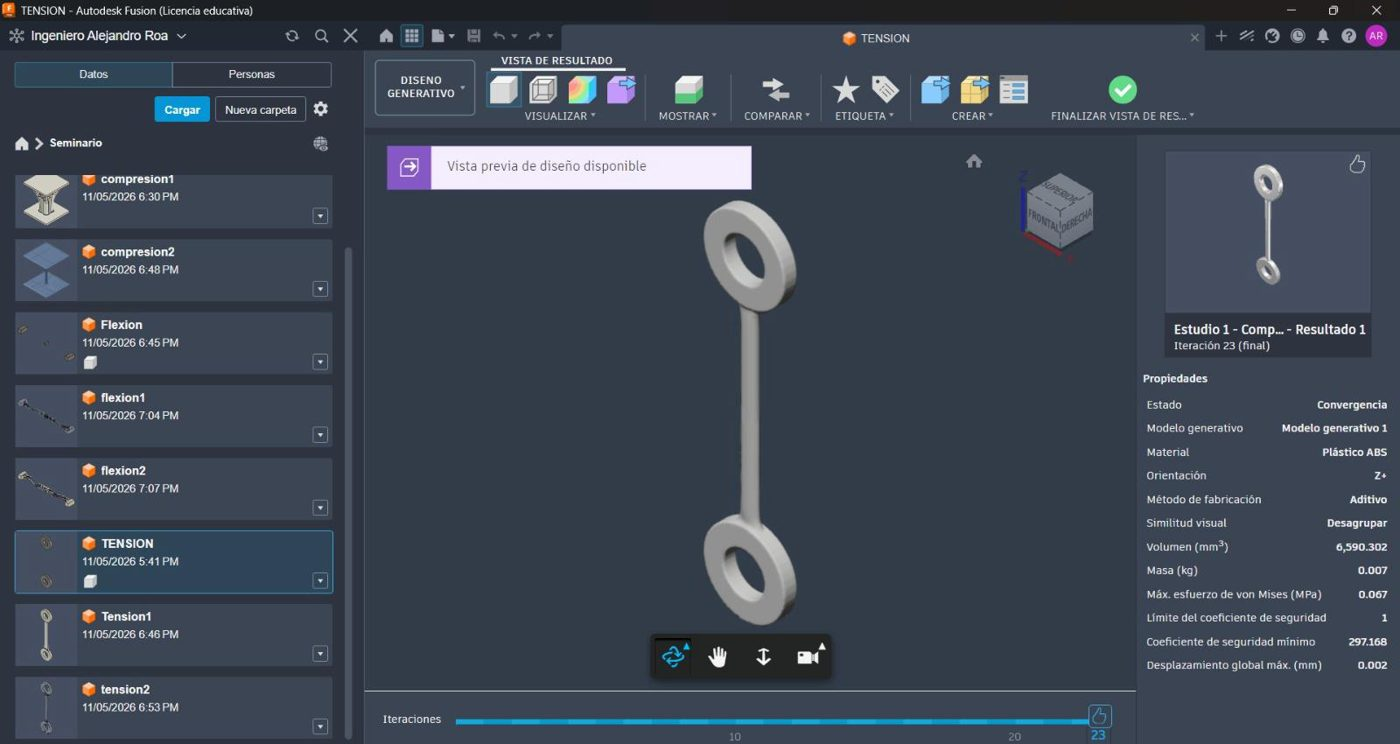
\includegraphics[width=\linewidth,height=0.20\textheight,keepaspectratio]{anexo/p20_0.jpg}\end{subfigure}\par\smallskip
\begin{subfigure}[t]{0.48\textwidth}\centering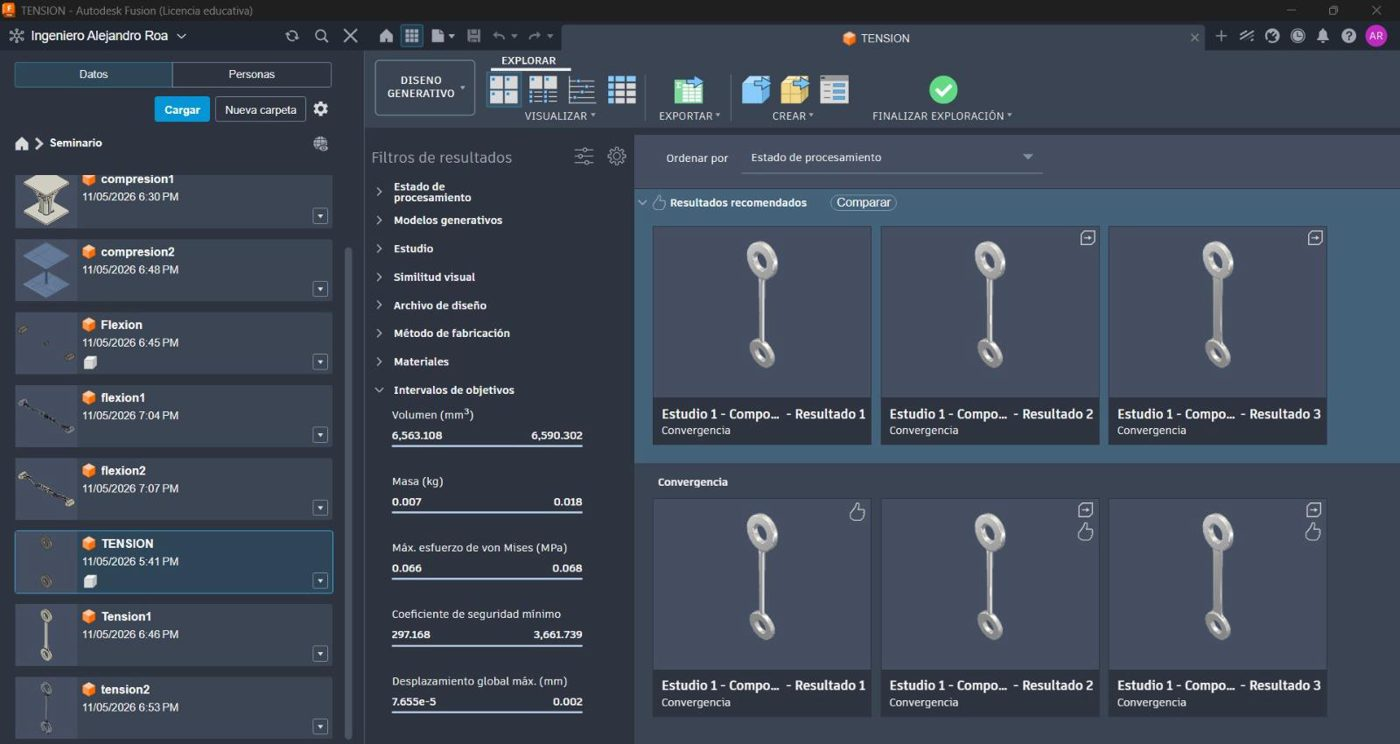
\includegraphics[width=\linewidth,height=0.20\textheight,keepaspectratio]{anexo/p20_1.jpg}\end{subfigure}\hfill
\caption{Diseño generativo de la pieza de tensión en Fusion 360: definición de geometrías y cargas, forma inicial y alternativas generadas.}
\par\footnotesize\textit{Nota.} Elaboración propia. Documento original, páginas 18 a 20.
\end{figure}
\begin{figure}[!htbp]\centering
\begin{subfigure}[t]{0.48\textwidth}\centering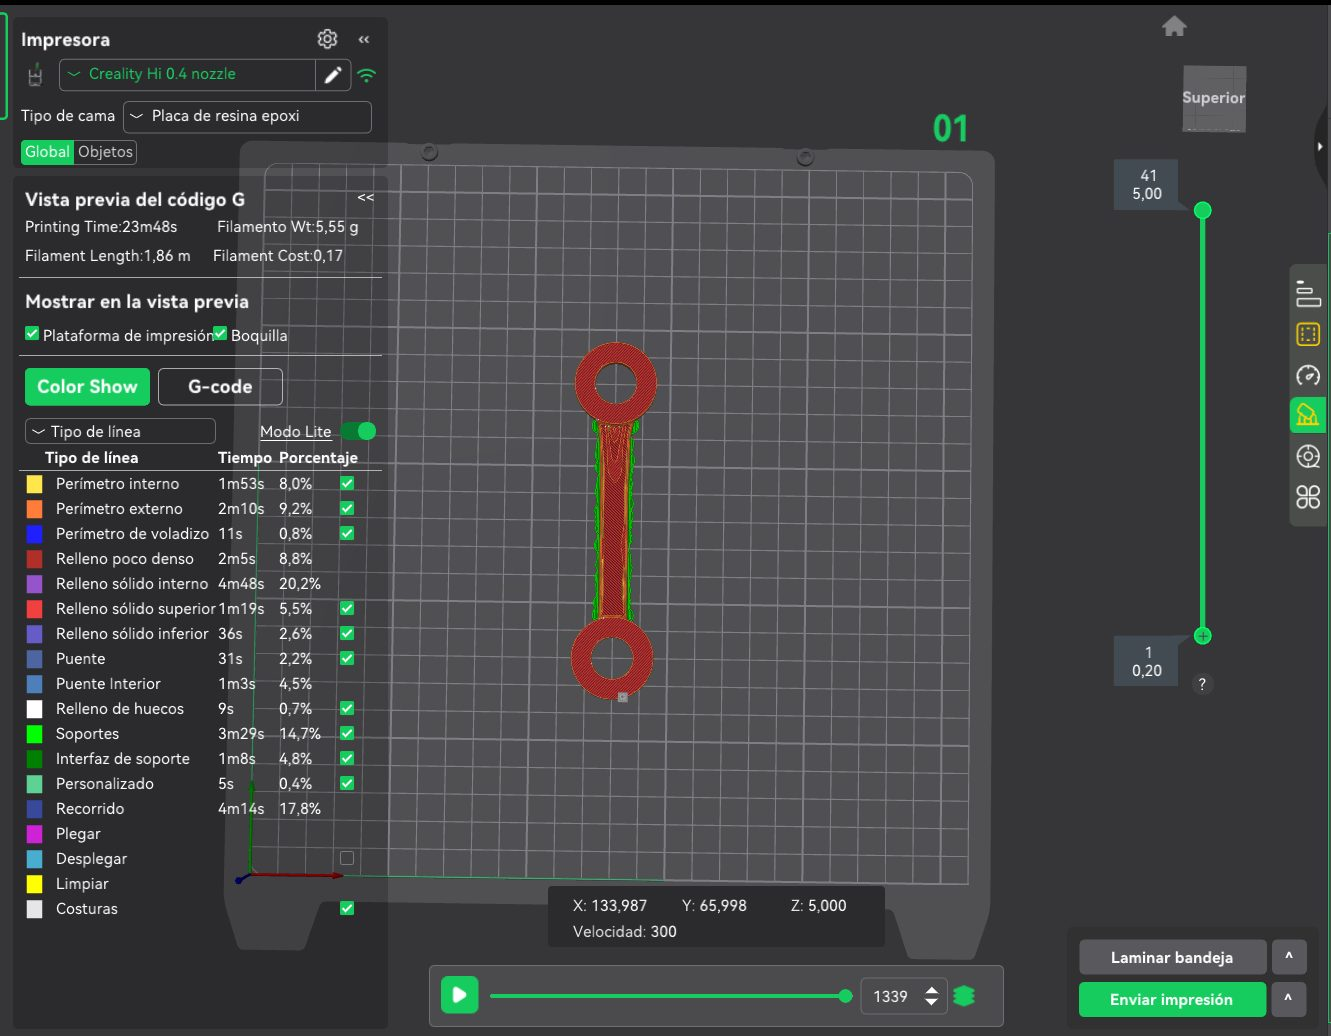
\includegraphics[width=\linewidth,height=0.28\textheight,keepaspectratio]{anexo/p21_0.jpg}\end{subfigure}\hfill
\begin{subfigure}[t]{0.48\textwidth}\centering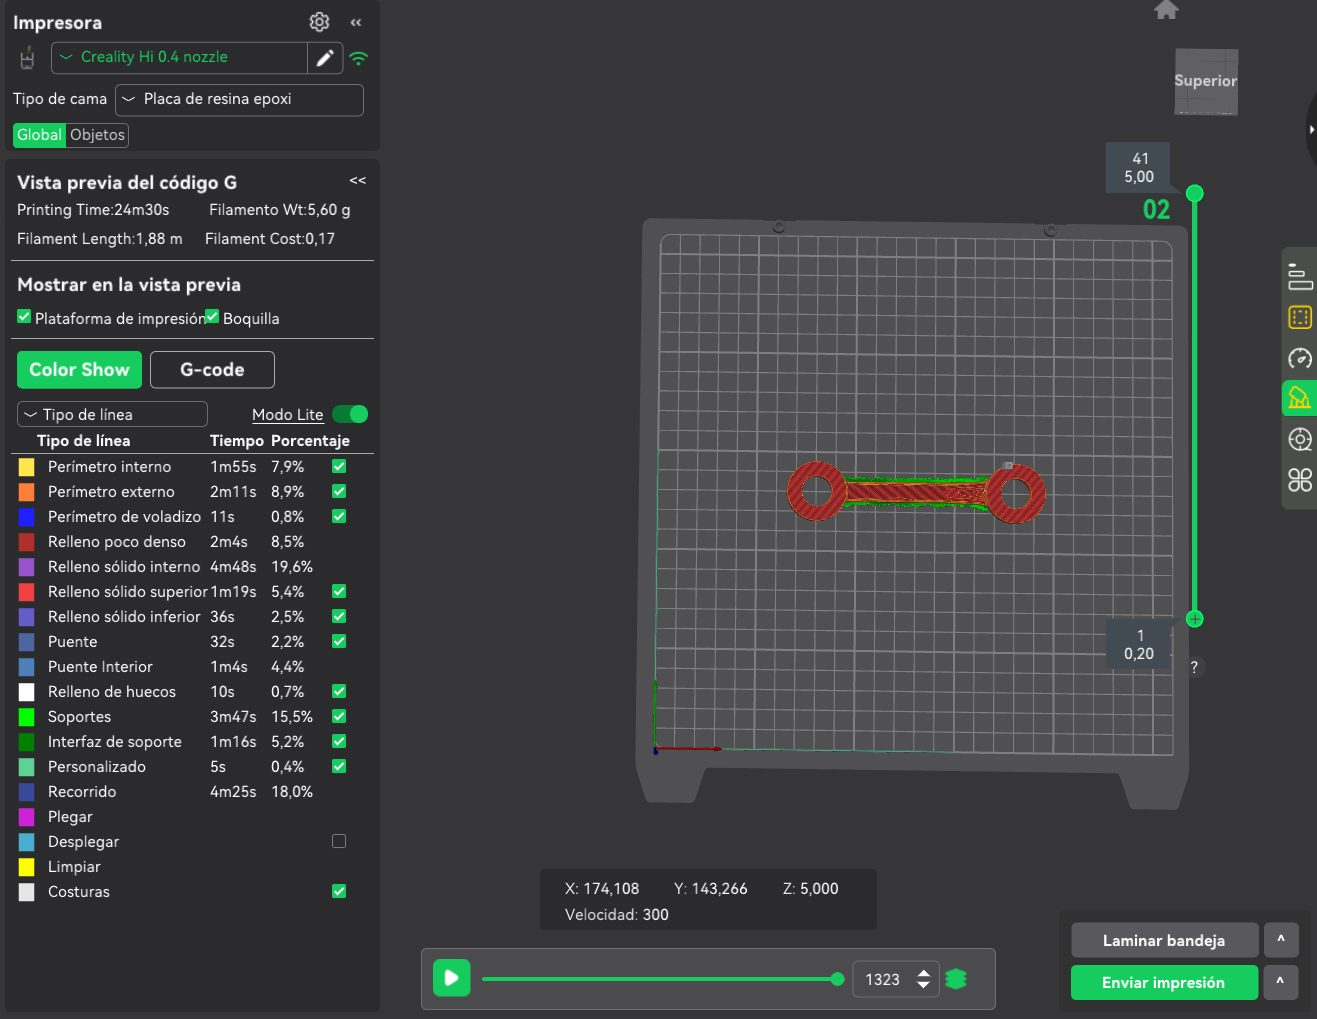
\includegraphics[width=\linewidth,height=0.28\textheight,keepaspectratio]{anexo/p22_0.jpg}\end{subfigure}\par\smallskip
\begin{subfigure}[t]{0.48\textwidth}\centering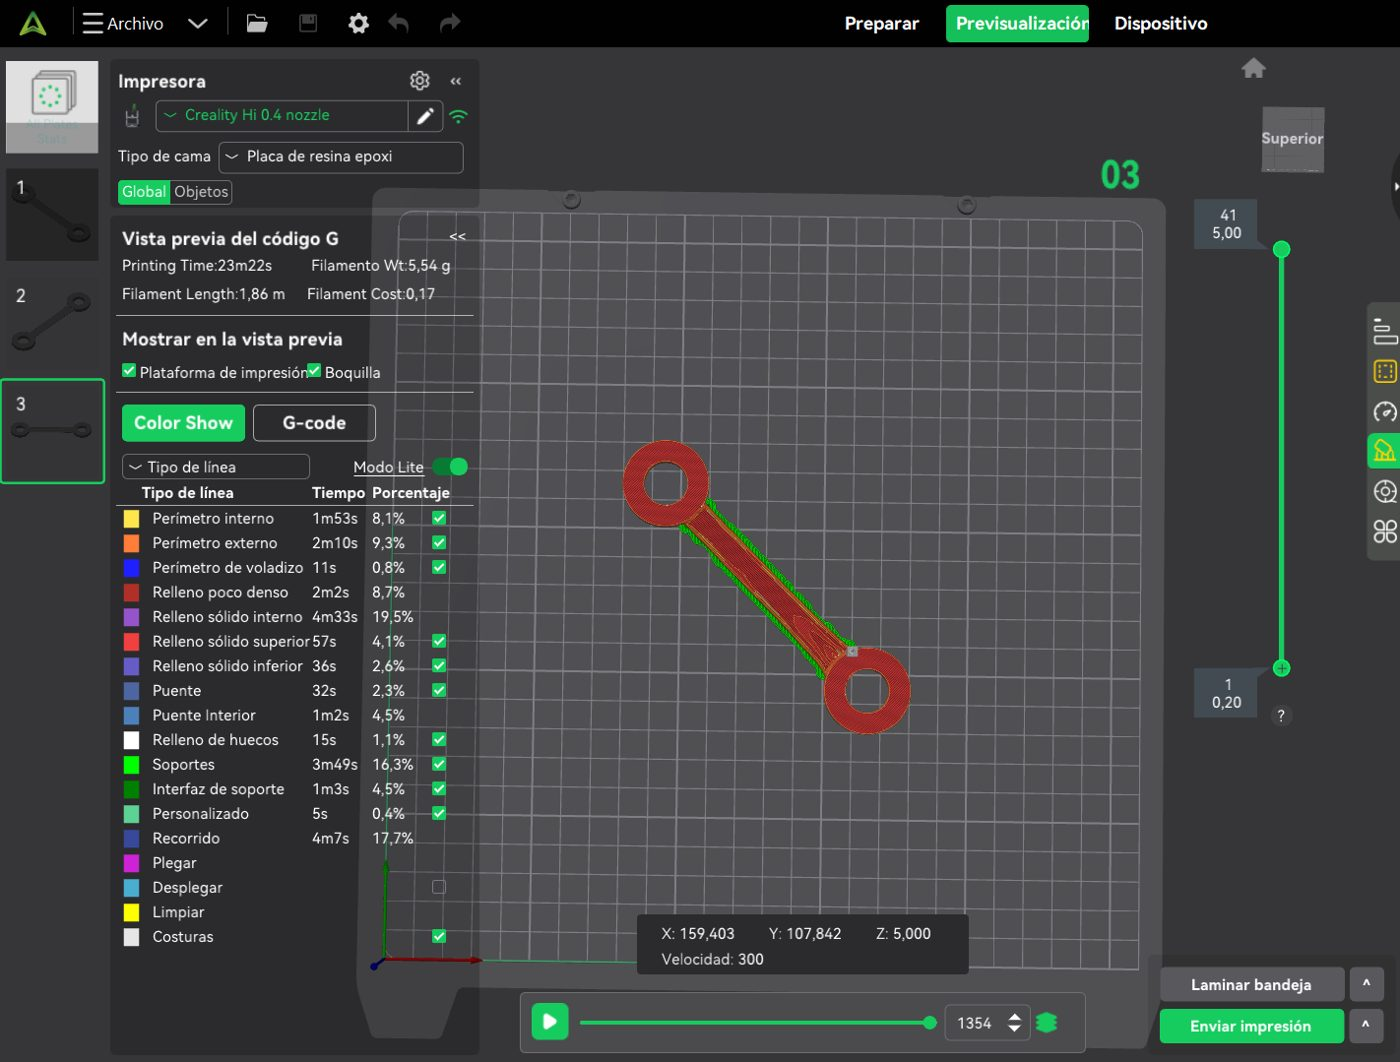
\includegraphics[width=\linewidth,height=0.28\textheight,keepaspectratio]{anexo/p23_0.jpg}\end{subfigure}\hfill
\begin{subfigure}[t]{0.48\textwidth}\centering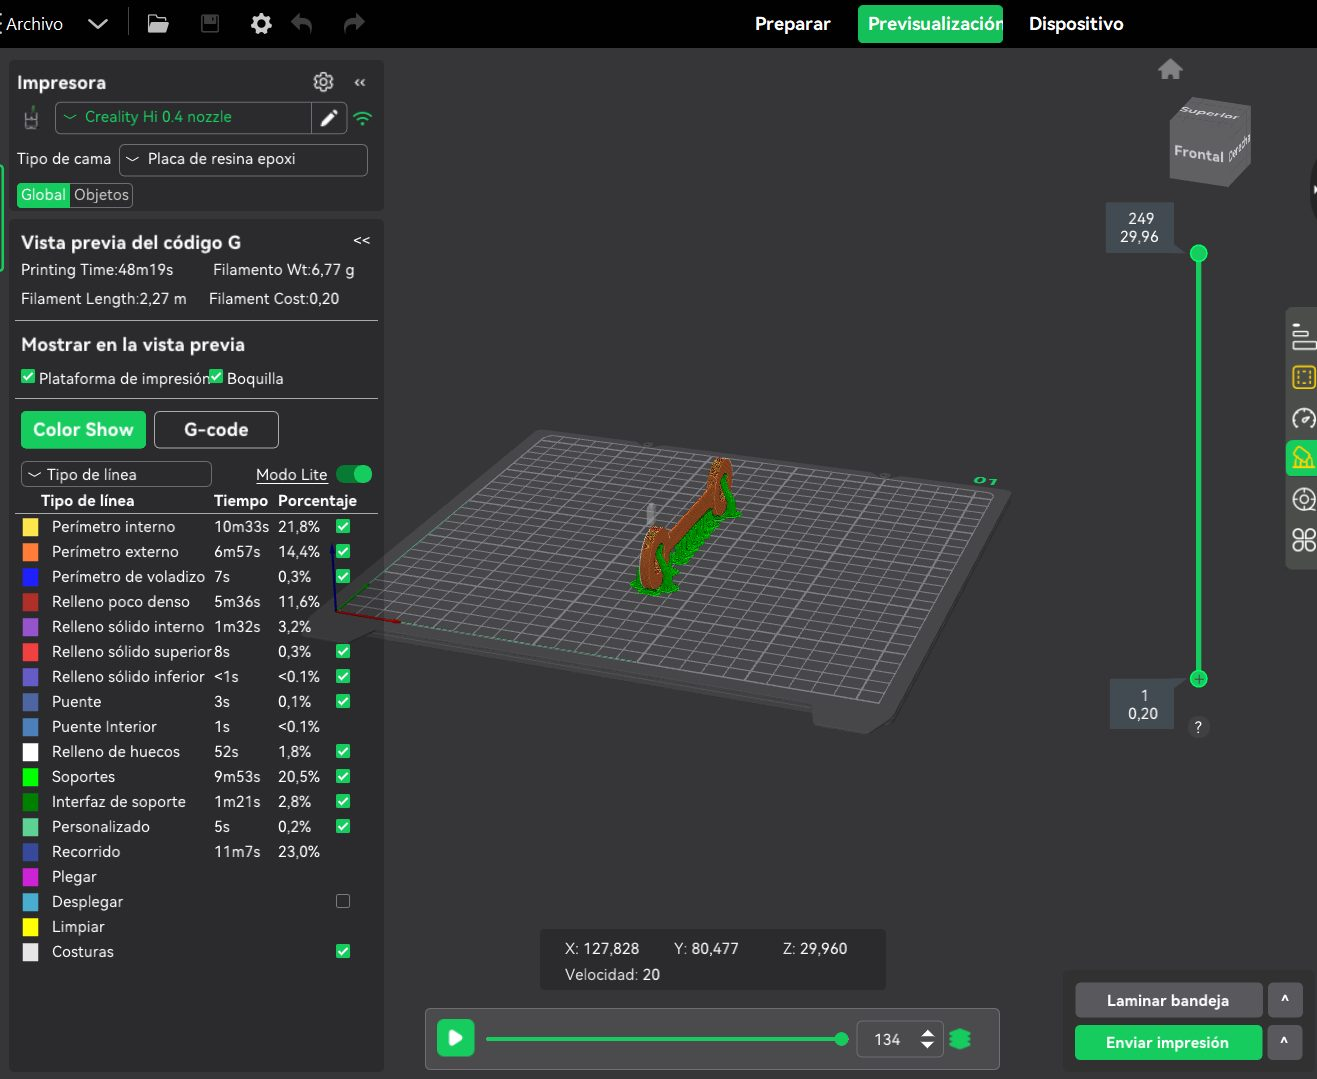
\includegraphics[width=\linewidth,height=0.28\textheight,keepaspectratio]{anexo/p24_0.jpg}\end{subfigure}\par\smallskip
\caption{Vistas de laminado en Creality Print con distintas orientaciones (1 de 3).}
\par\footnotesize\textit{Nota.} Elaboración propia. Documento original, páginas 21 a 24.
\end{figure}
\begin{figure}[!htbp]\centering
\begin{subfigure}[t]{0.48\textwidth}\centering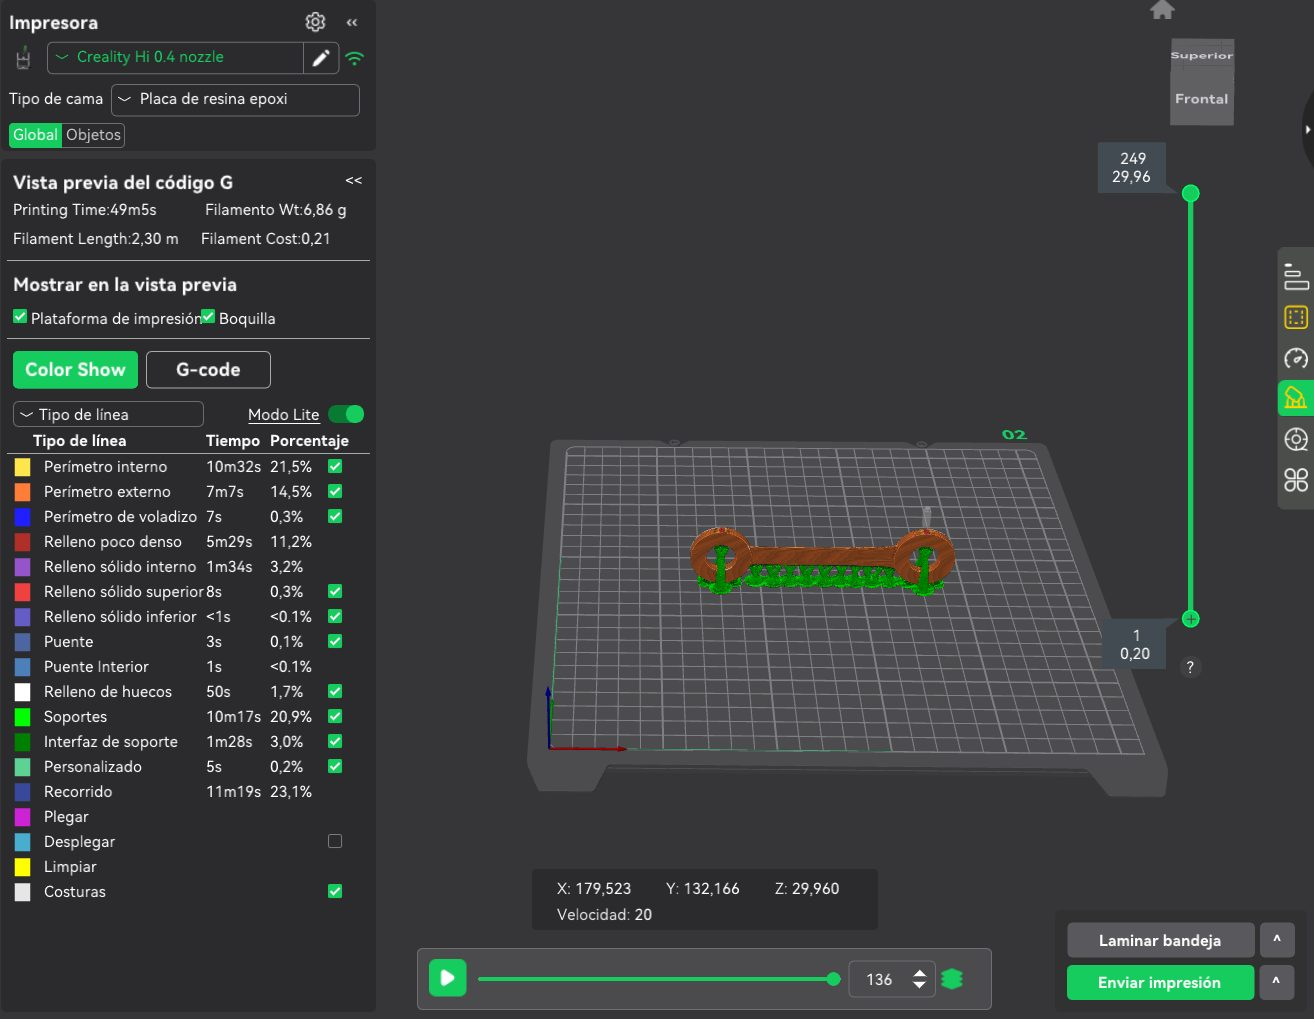
\includegraphics[width=\linewidth,height=0.28\textheight,keepaspectratio]{anexo/p25_0.jpg}\end{subfigure}\hfill
\begin{subfigure}[t]{0.48\textwidth}\centering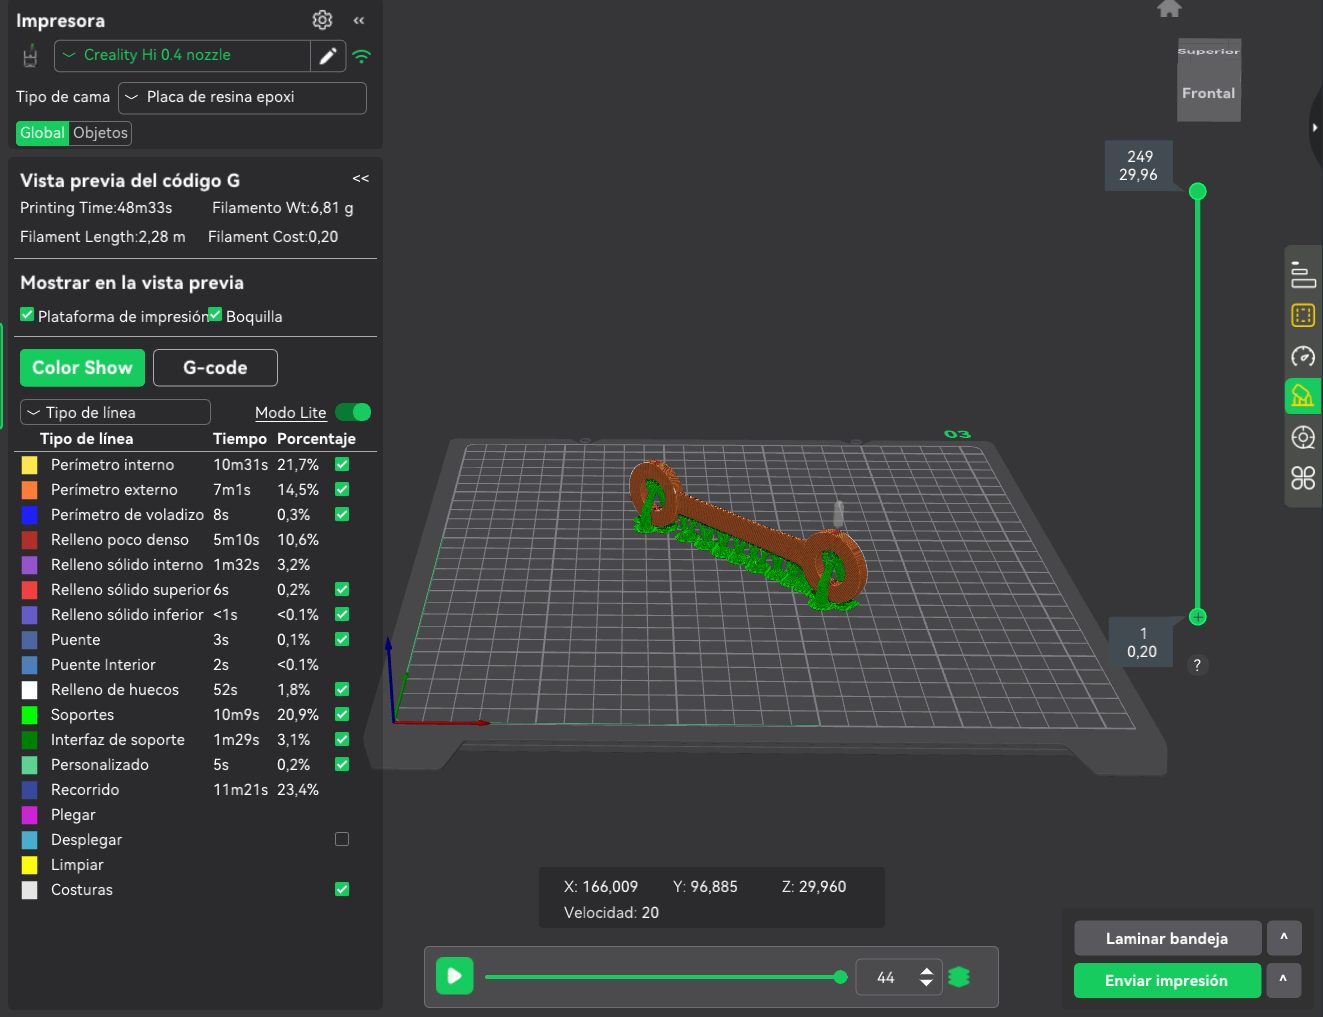
\includegraphics[width=\linewidth,height=0.28\textheight,keepaspectratio]{anexo/p26_0.jpg}\end{subfigure}\par\smallskip
\begin{subfigure}[t]{0.48\textwidth}\centering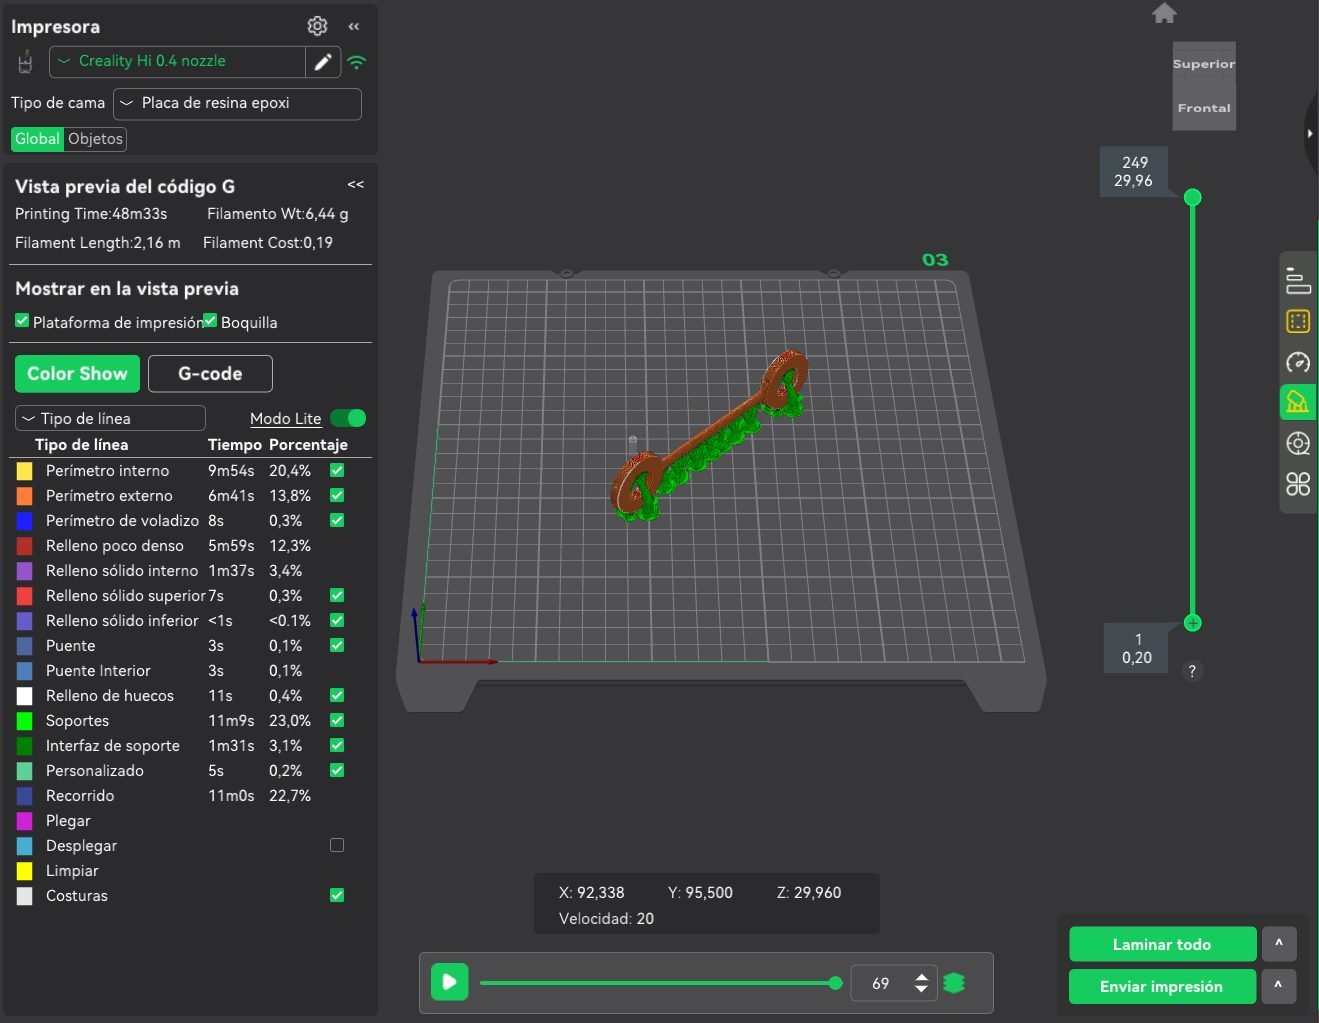
\includegraphics[width=\linewidth,height=0.28\textheight,keepaspectratio]{anexo/p27_0.jpg}\end{subfigure}\hfill
\begin{subfigure}[t]{0.48\textwidth}\centering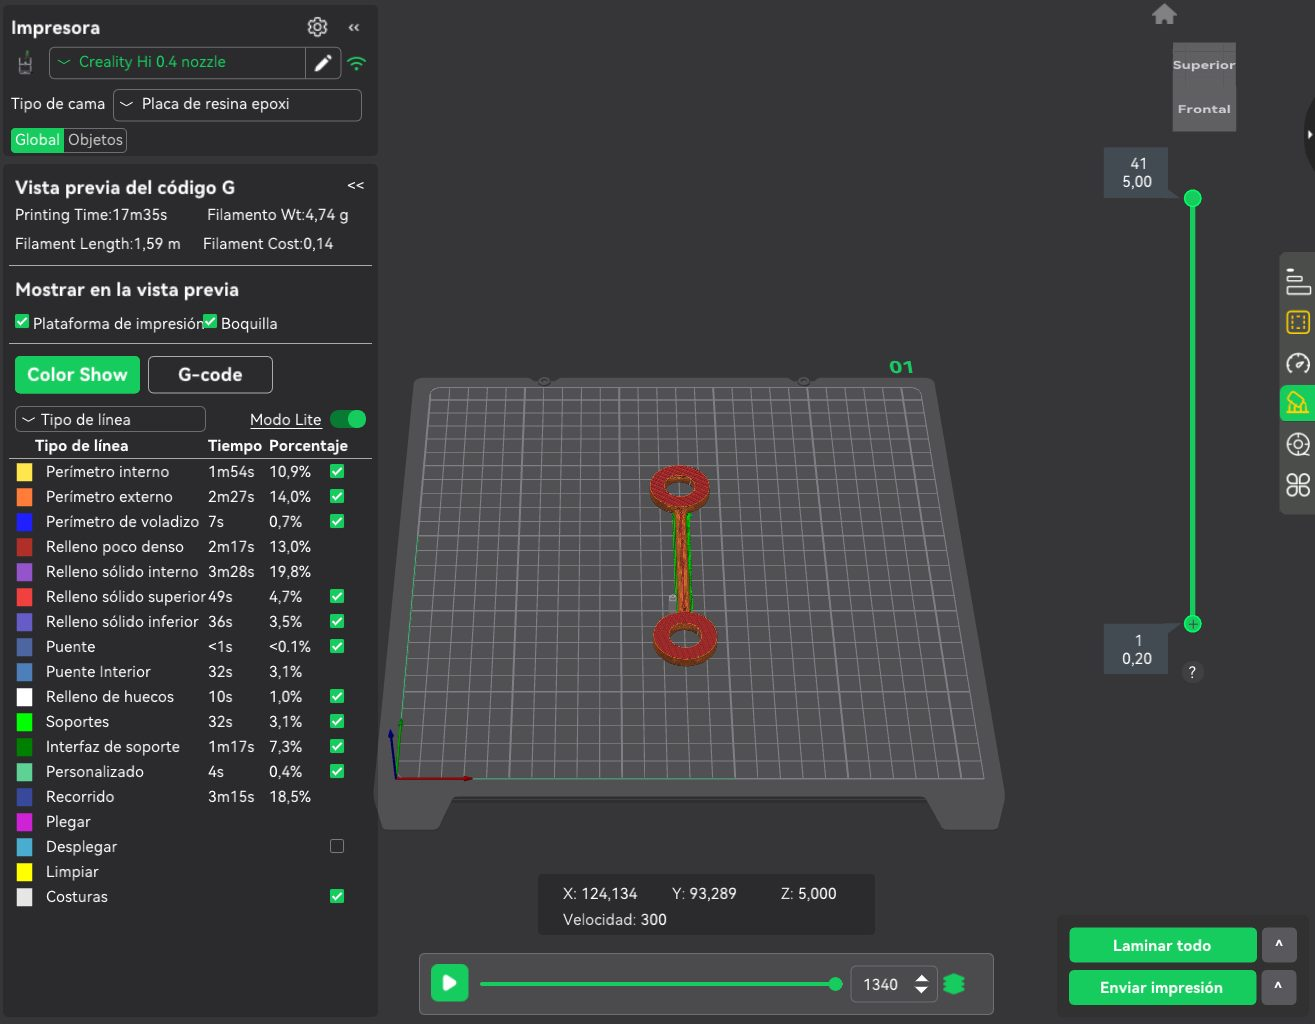
\includegraphics[width=\linewidth,height=0.28\textheight,keepaspectratio]{anexo/p28_0.jpg}\end{subfigure}\par\smallskip
\caption{Vistas de laminado en Creality Print con distintas orientaciones (2 de 3).}
\par\footnotesize\textit{Nota.} Elaboración propia. Documento original, páginas 25 a 28.
\end{figure}
\begin{figure}[!htbp]\centering
\begin{subfigure}[t]{0.48\textwidth}\centering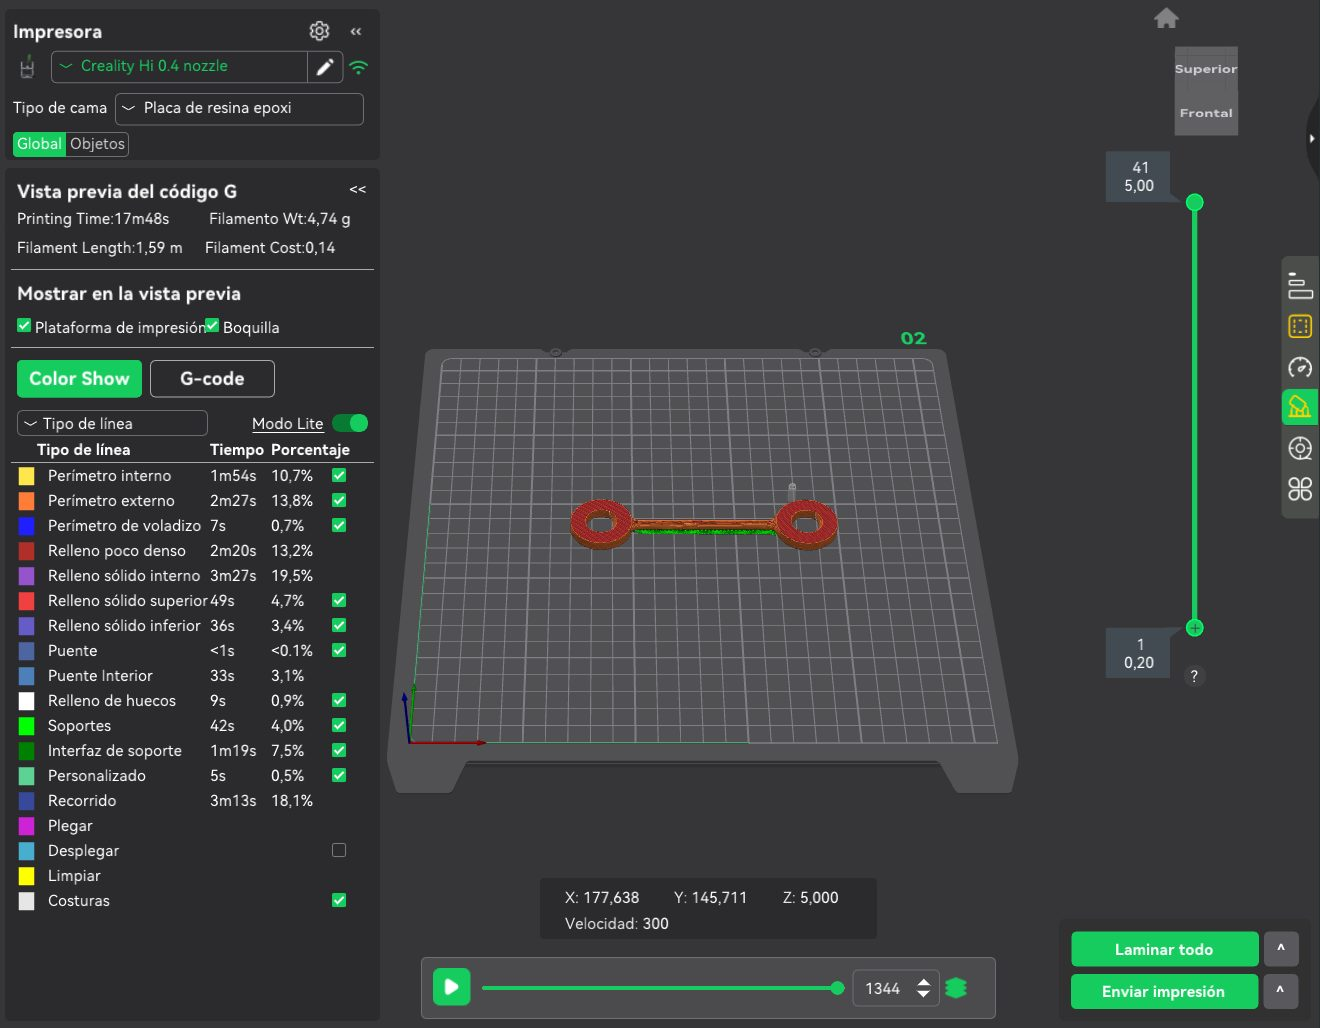
\includegraphics[width=\linewidth,height=0.28\textheight,keepaspectratio]{anexo/p29_0.jpg}\end{subfigure}\hfill
\begin{subfigure}[t]{0.48\textwidth}\centering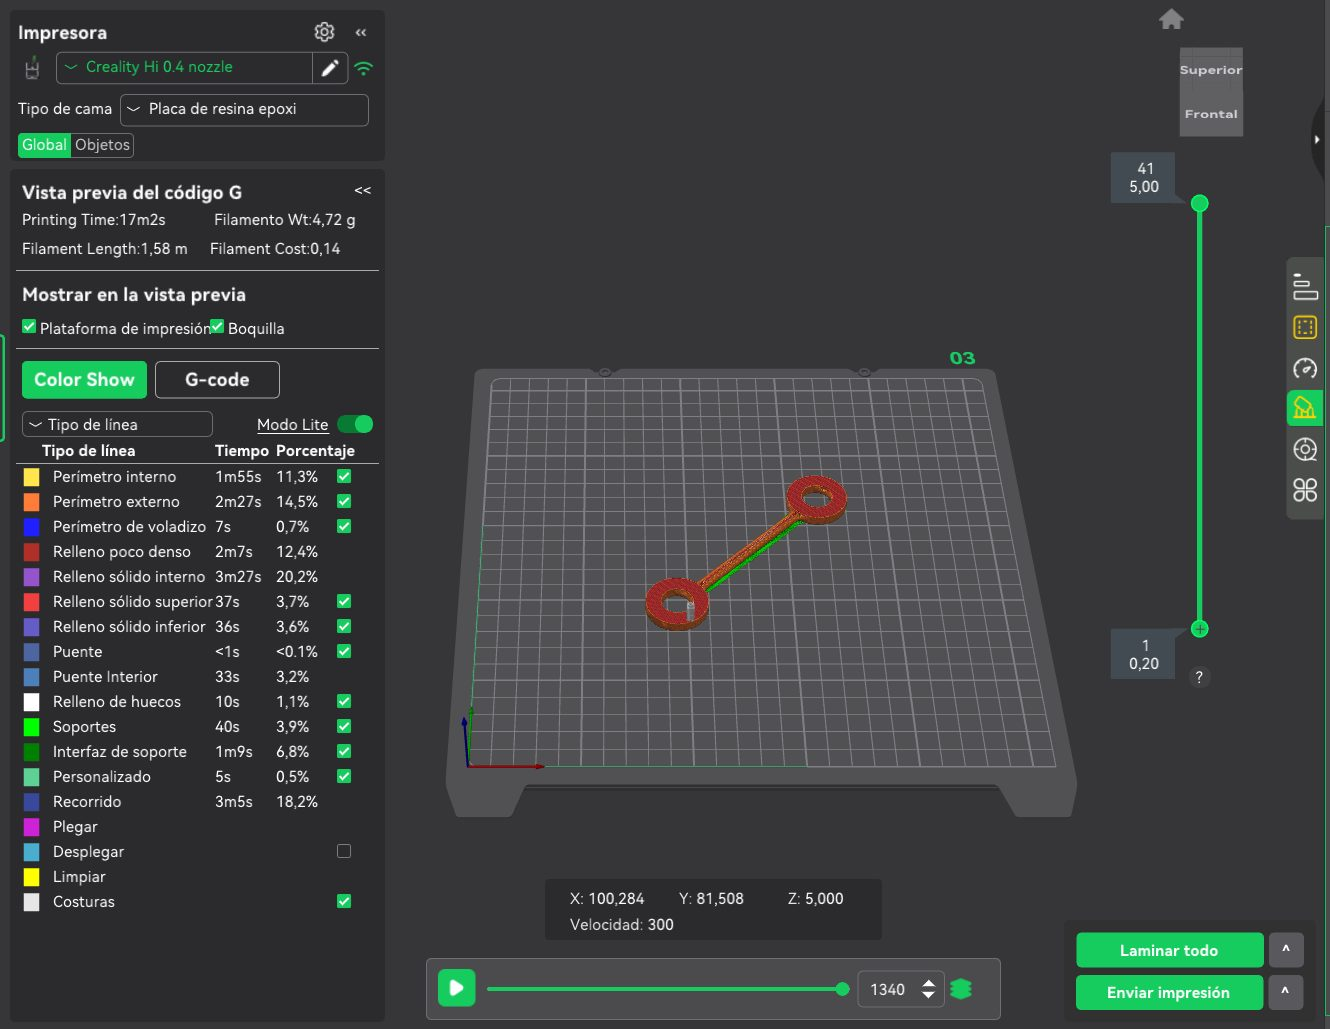
\includegraphics[width=\linewidth,height=0.28\textheight,keepaspectratio]{anexo/p30_0.jpg}\end{subfigure}\par\smallskip
\begin{subfigure}[t]{0.48\textwidth}\centering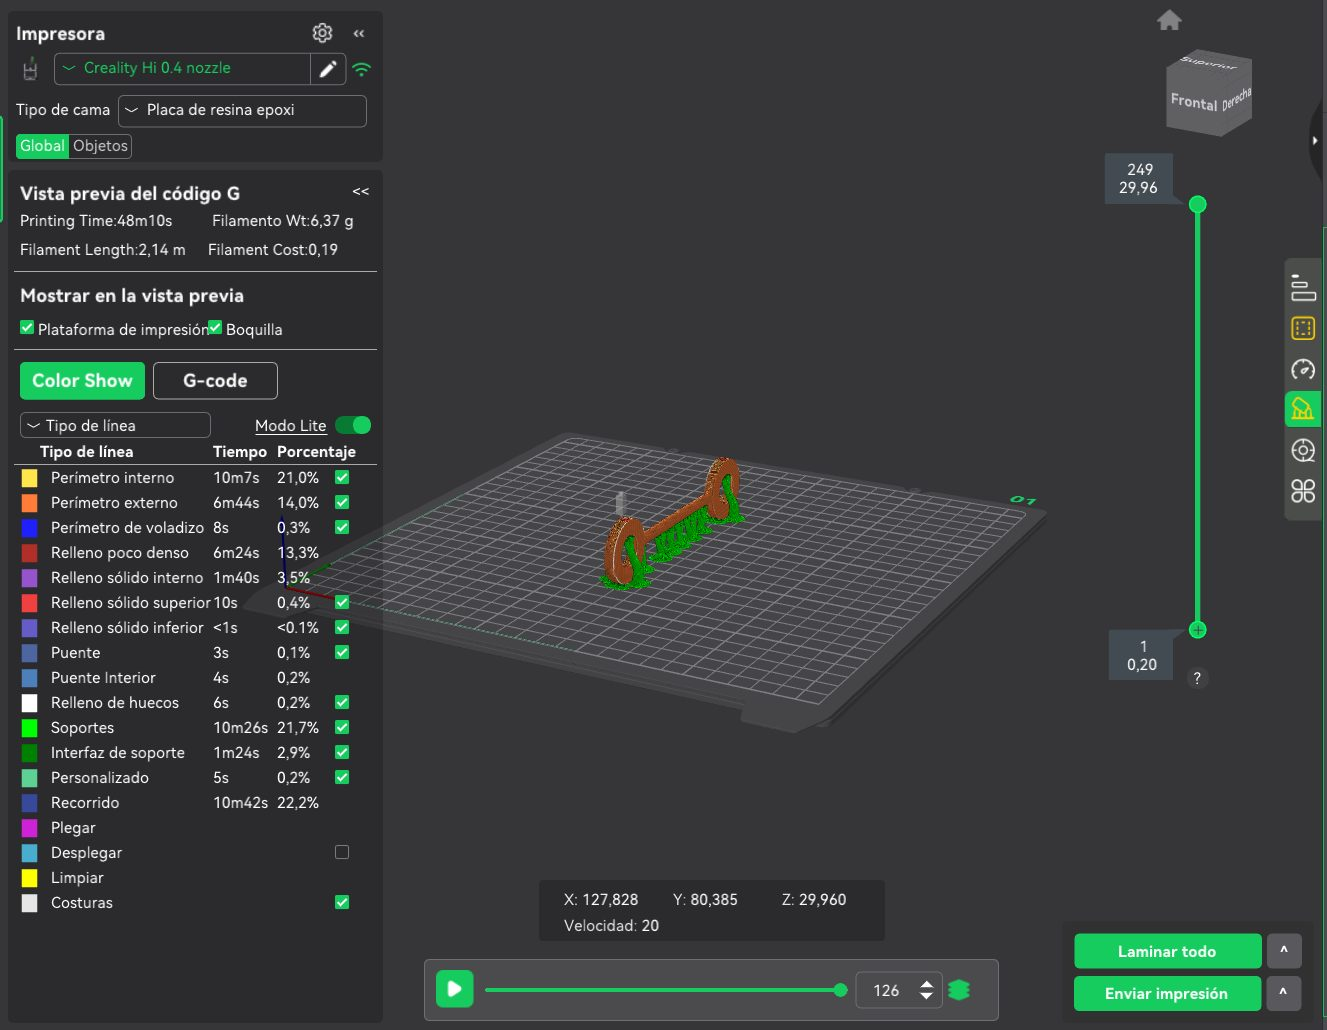
\includegraphics[width=\linewidth,height=0.28\textheight,keepaspectratio]{anexo/p31_0.jpg}\end{subfigure}\hfill
\begin{subfigure}[t]{0.48\textwidth}\centering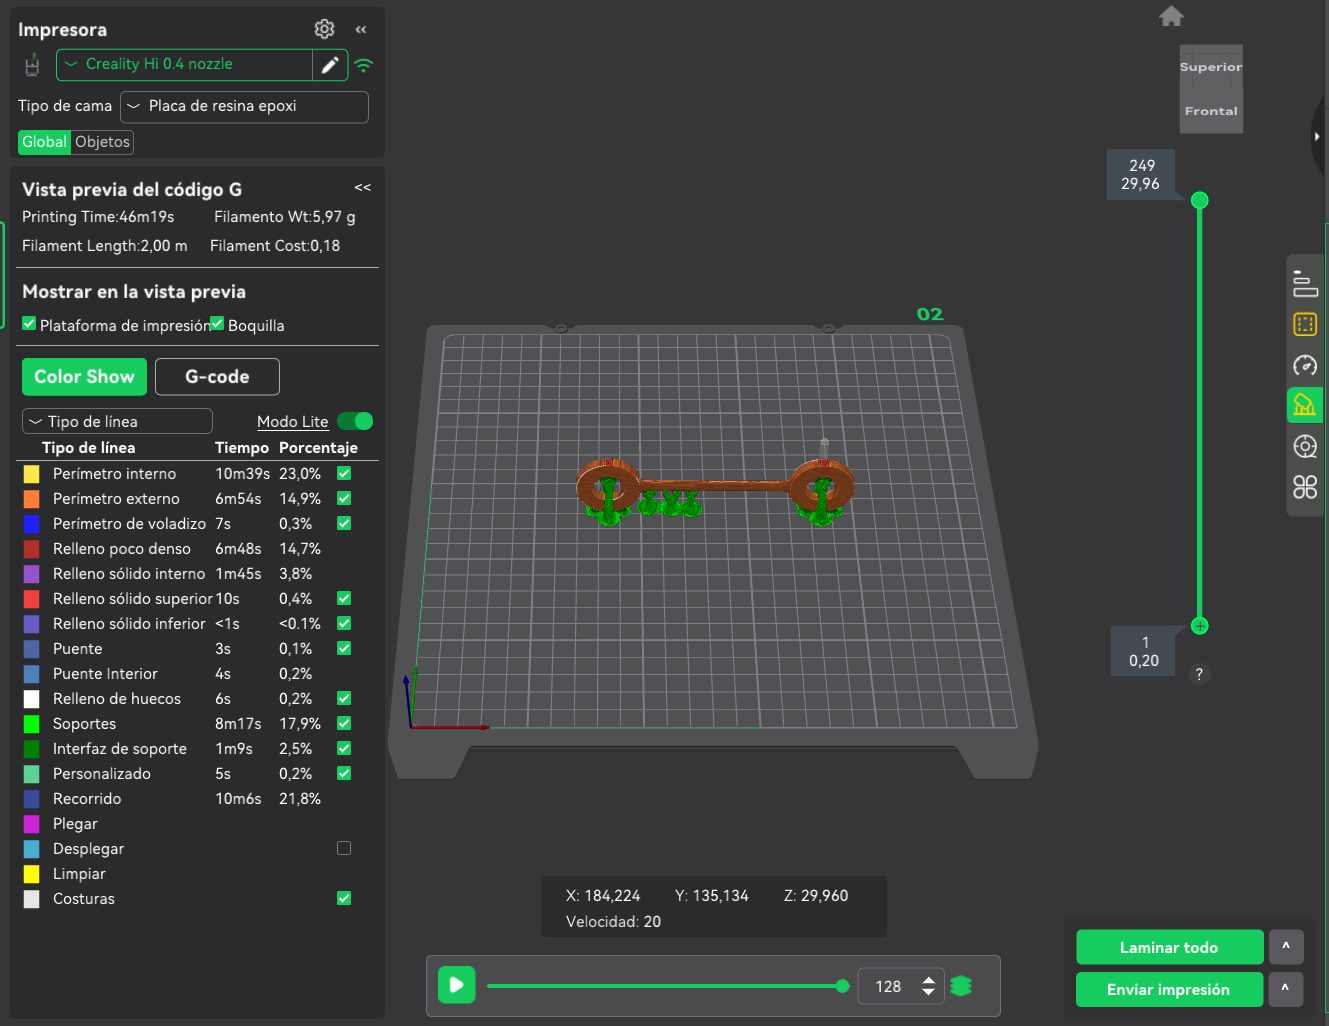
\includegraphics[width=\linewidth,height=0.28\textheight,keepaspectratio]{anexo/p32_0.jpg}\end{subfigure}\par\smallskip
\caption{Vistas de laminado en Creality Print con distintas orientaciones (3 de 3).}
\par\footnotesize\textit{Nota.} Elaboración propia. Documento original, páginas 29 a 32.
\end{figure}
\begin{figure}[!htbp]\centering
\begin{subfigure}[t]{0.48\textwidth}\centering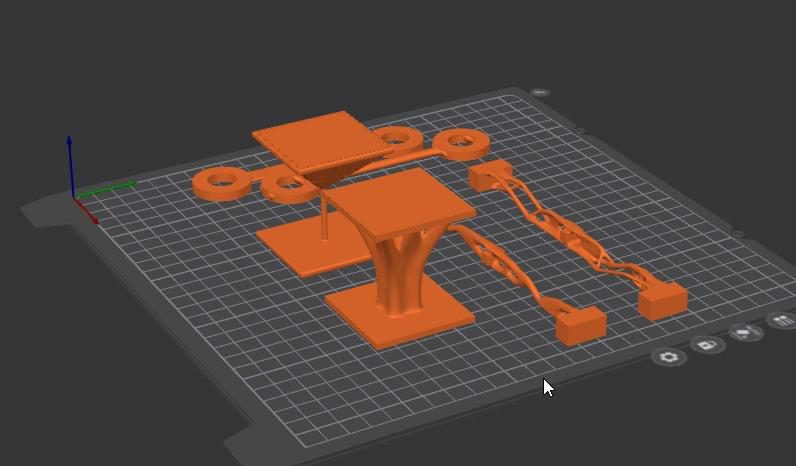
\includegraphics[width=\linewidth,height=0.28\textheight,keepaspectratio]{anexo/p33_0.jpg}\end{subfigure}\hfill
\begin{subfigure}[t]{0.48\textwidth}\centering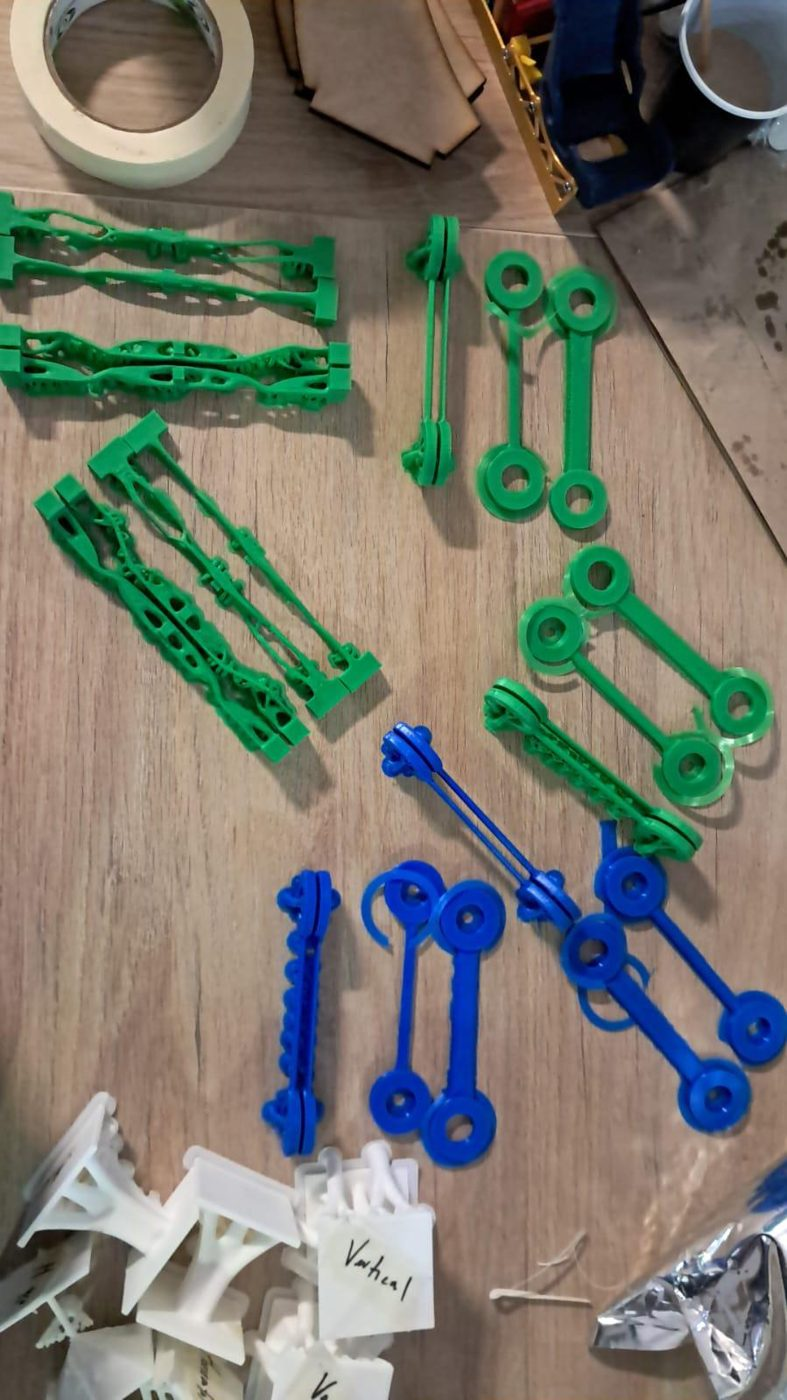
\includegraphics[width=\linewidth,height=0.28\textheight,keepaspectratio]{anexo/p33_1.jpg}\end{subfigure}\par\smallskip
\begin{subfigure}[t]{0.48\textwidth}\centering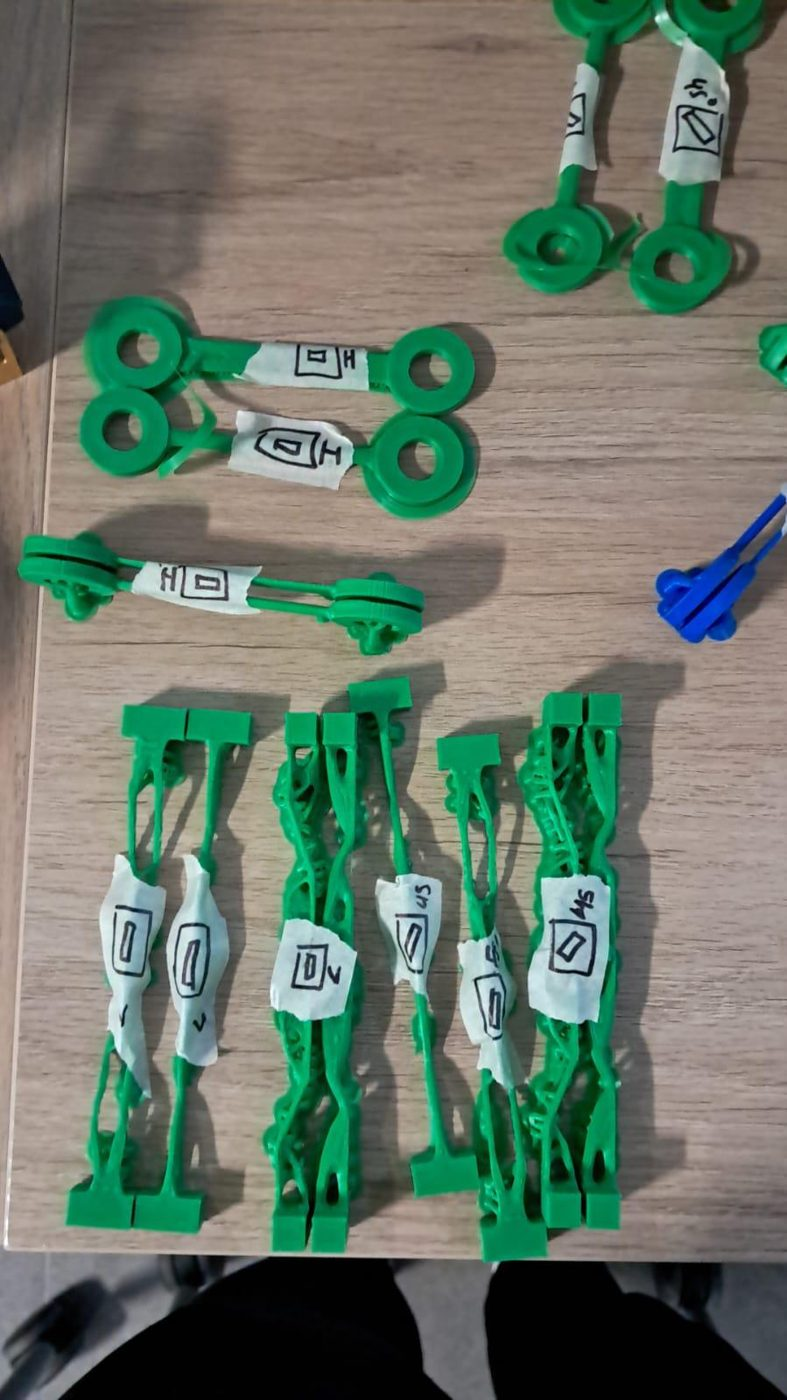
\includegraphics[width=\linewidth,height=0.28\textheight,keepaspectratio]{anexo/p34_0.jpg}\end{subfigure}\hfill
\begin{subfigure}[t]{0.48\textwidth}\centering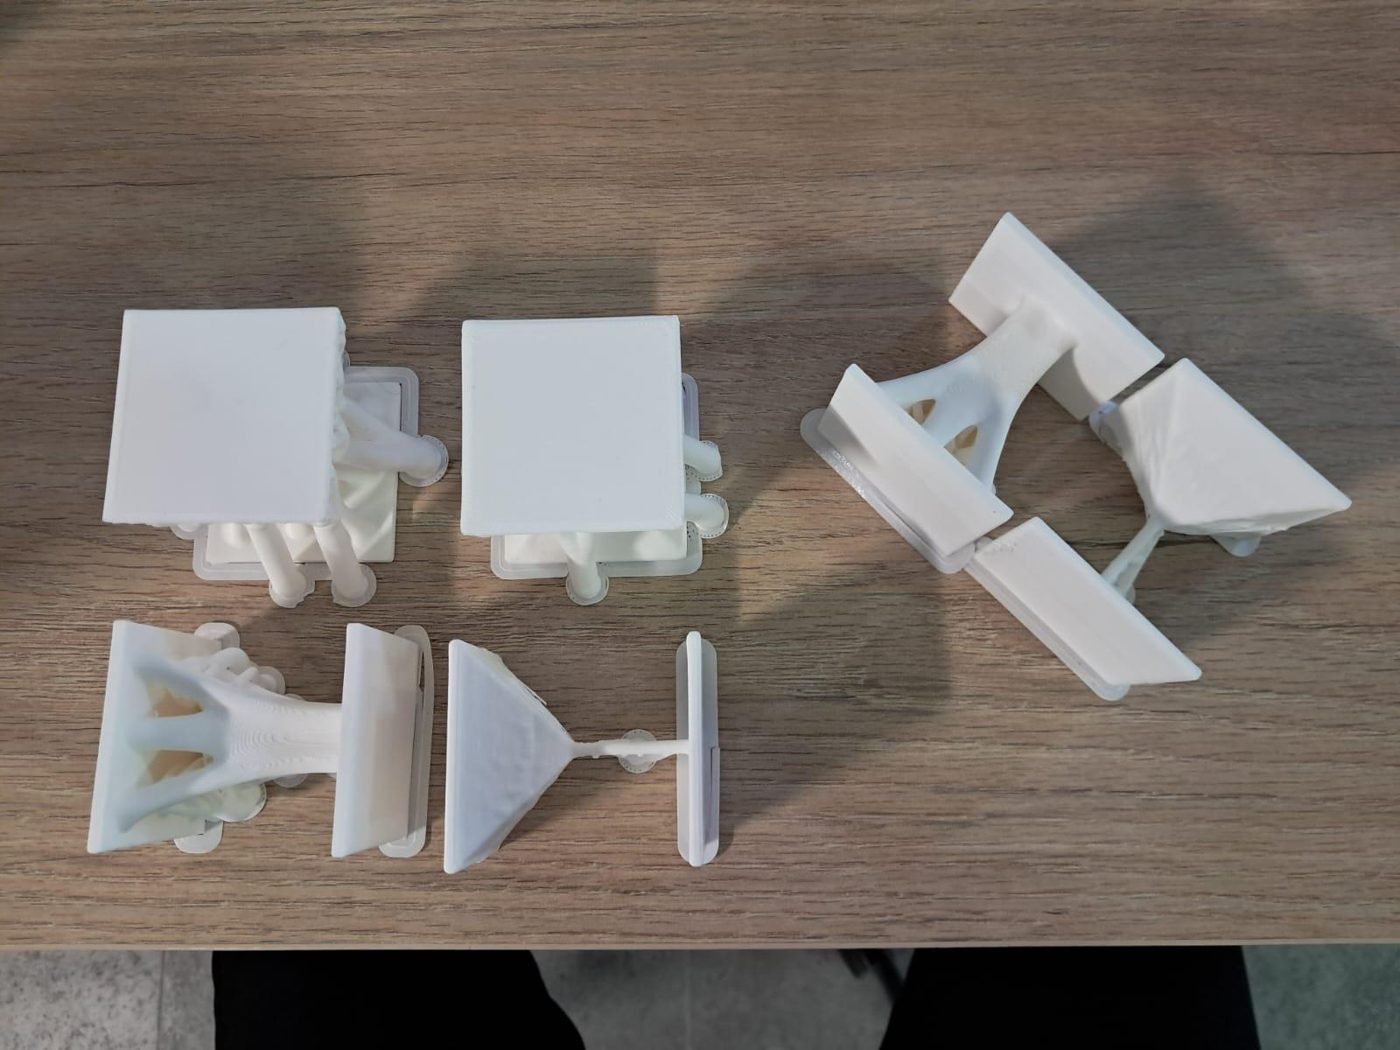
\includegraphics[width=\linewidth,height=0.28\textheight,keepaspectratio]{anexo/p34_1.jpg}\end{subfigure}\par\smallskip
\caption{Distribución de las piezas en la cama de impresión y piezas fabricadas.}
\par\footnotesize\textit{Nota.} Elaboración propia. Documento original, páginas 33 y 34.
\end{figure}
\endgroup
